\documentclass{beamer}
%
% Choose how your presentation looks.
%
% For more themes, color themes and font themes, see:
% http://deic.uab.es/~iblanes/beamer_gallery/index_by_theme.html
%
\mode<presentation>
{
  \usetheme{default}      % or try Darmstadt, Madrid, Warsaw, ...
  \usecolortheme{default} % or try albatross, beaver, crane, ...
  \usefonttheme{default}  % or try serif, structurebold, ...
  \setbeamertemplate{navigation symbols}{}
  \setbeamertemplate{caption}[numbered]
} 
\usepackage{amsthm}
\usepackage{polski}
\usepackage[utf8x]{inputenc}
\usepackage{enumitem}
\usepackage{epstopdf}
\title[Your Short Title]{Your Presentation}
\author{Andrzej Kokosza}
\date{Oblicze 2016}


\makeatletter
\newenvironment<>{proofs}[1][\proofname]{%
    \par
    \def\insertproofname{#1\@addpunct{.}}%
    \usebeamertemplate{proof begin}#2}
  {\usebeamertemplate{proof end}}
\makeatother


\newtheorem{definicja}{Definicja}
\newtheorem{przyklad}{Przykład}
\newtheorem{twierdzenie}{Twierdzenie}

\begin{document}

\begin{frame}
  \titlepage
\end{frame}

% Uncomment these lines for an automatically generated outline.
%\begin{frame}{Outline}
%  \tableofcontents
%\end{frame}

\section{Aksjomaty}

\begin{frame}{Aksjomaty}

\begin{figure}[!htb]
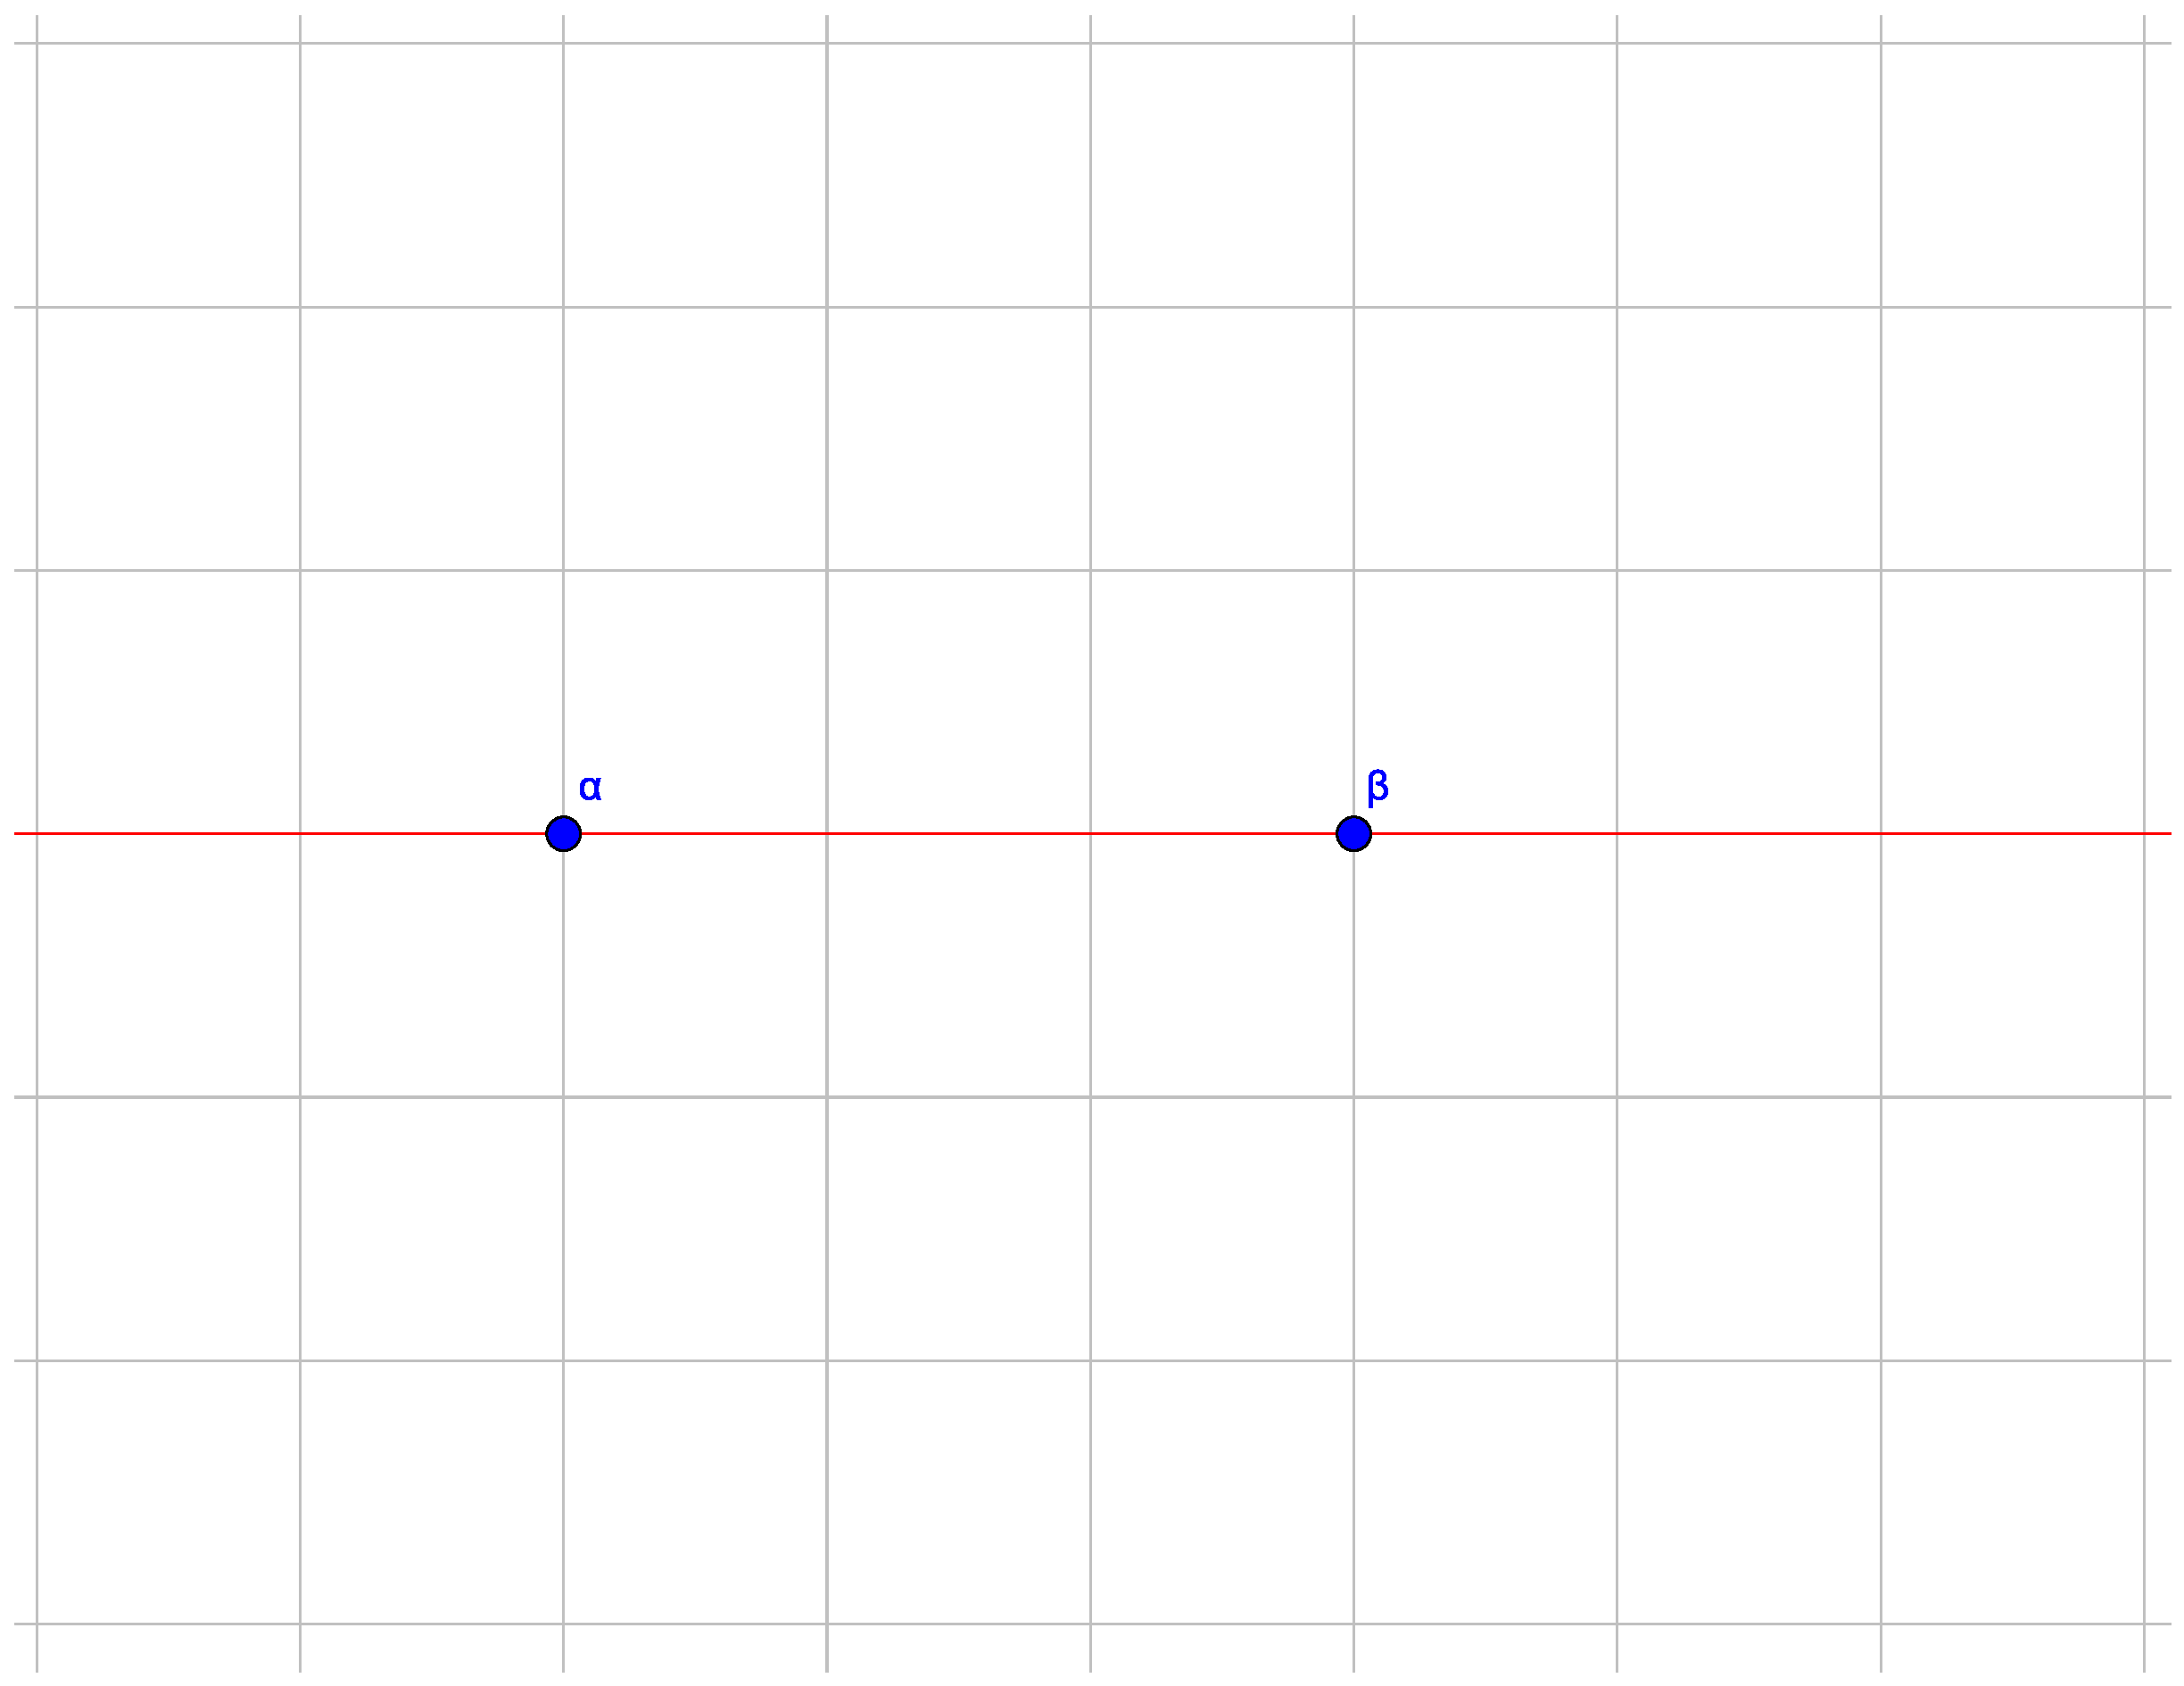
\includegraphics[scale=0.2]{C1.eps}
\label{fig:C1}
\end{figure}

\begin{block}{}
\centering
(C1)  Dwa punkty $\alpha\not=\beta$ można połączyć prostą.
\end{block}

\end{frame}


\begin{frame}{Aksjomaty}

\begin{figure}[!htb]
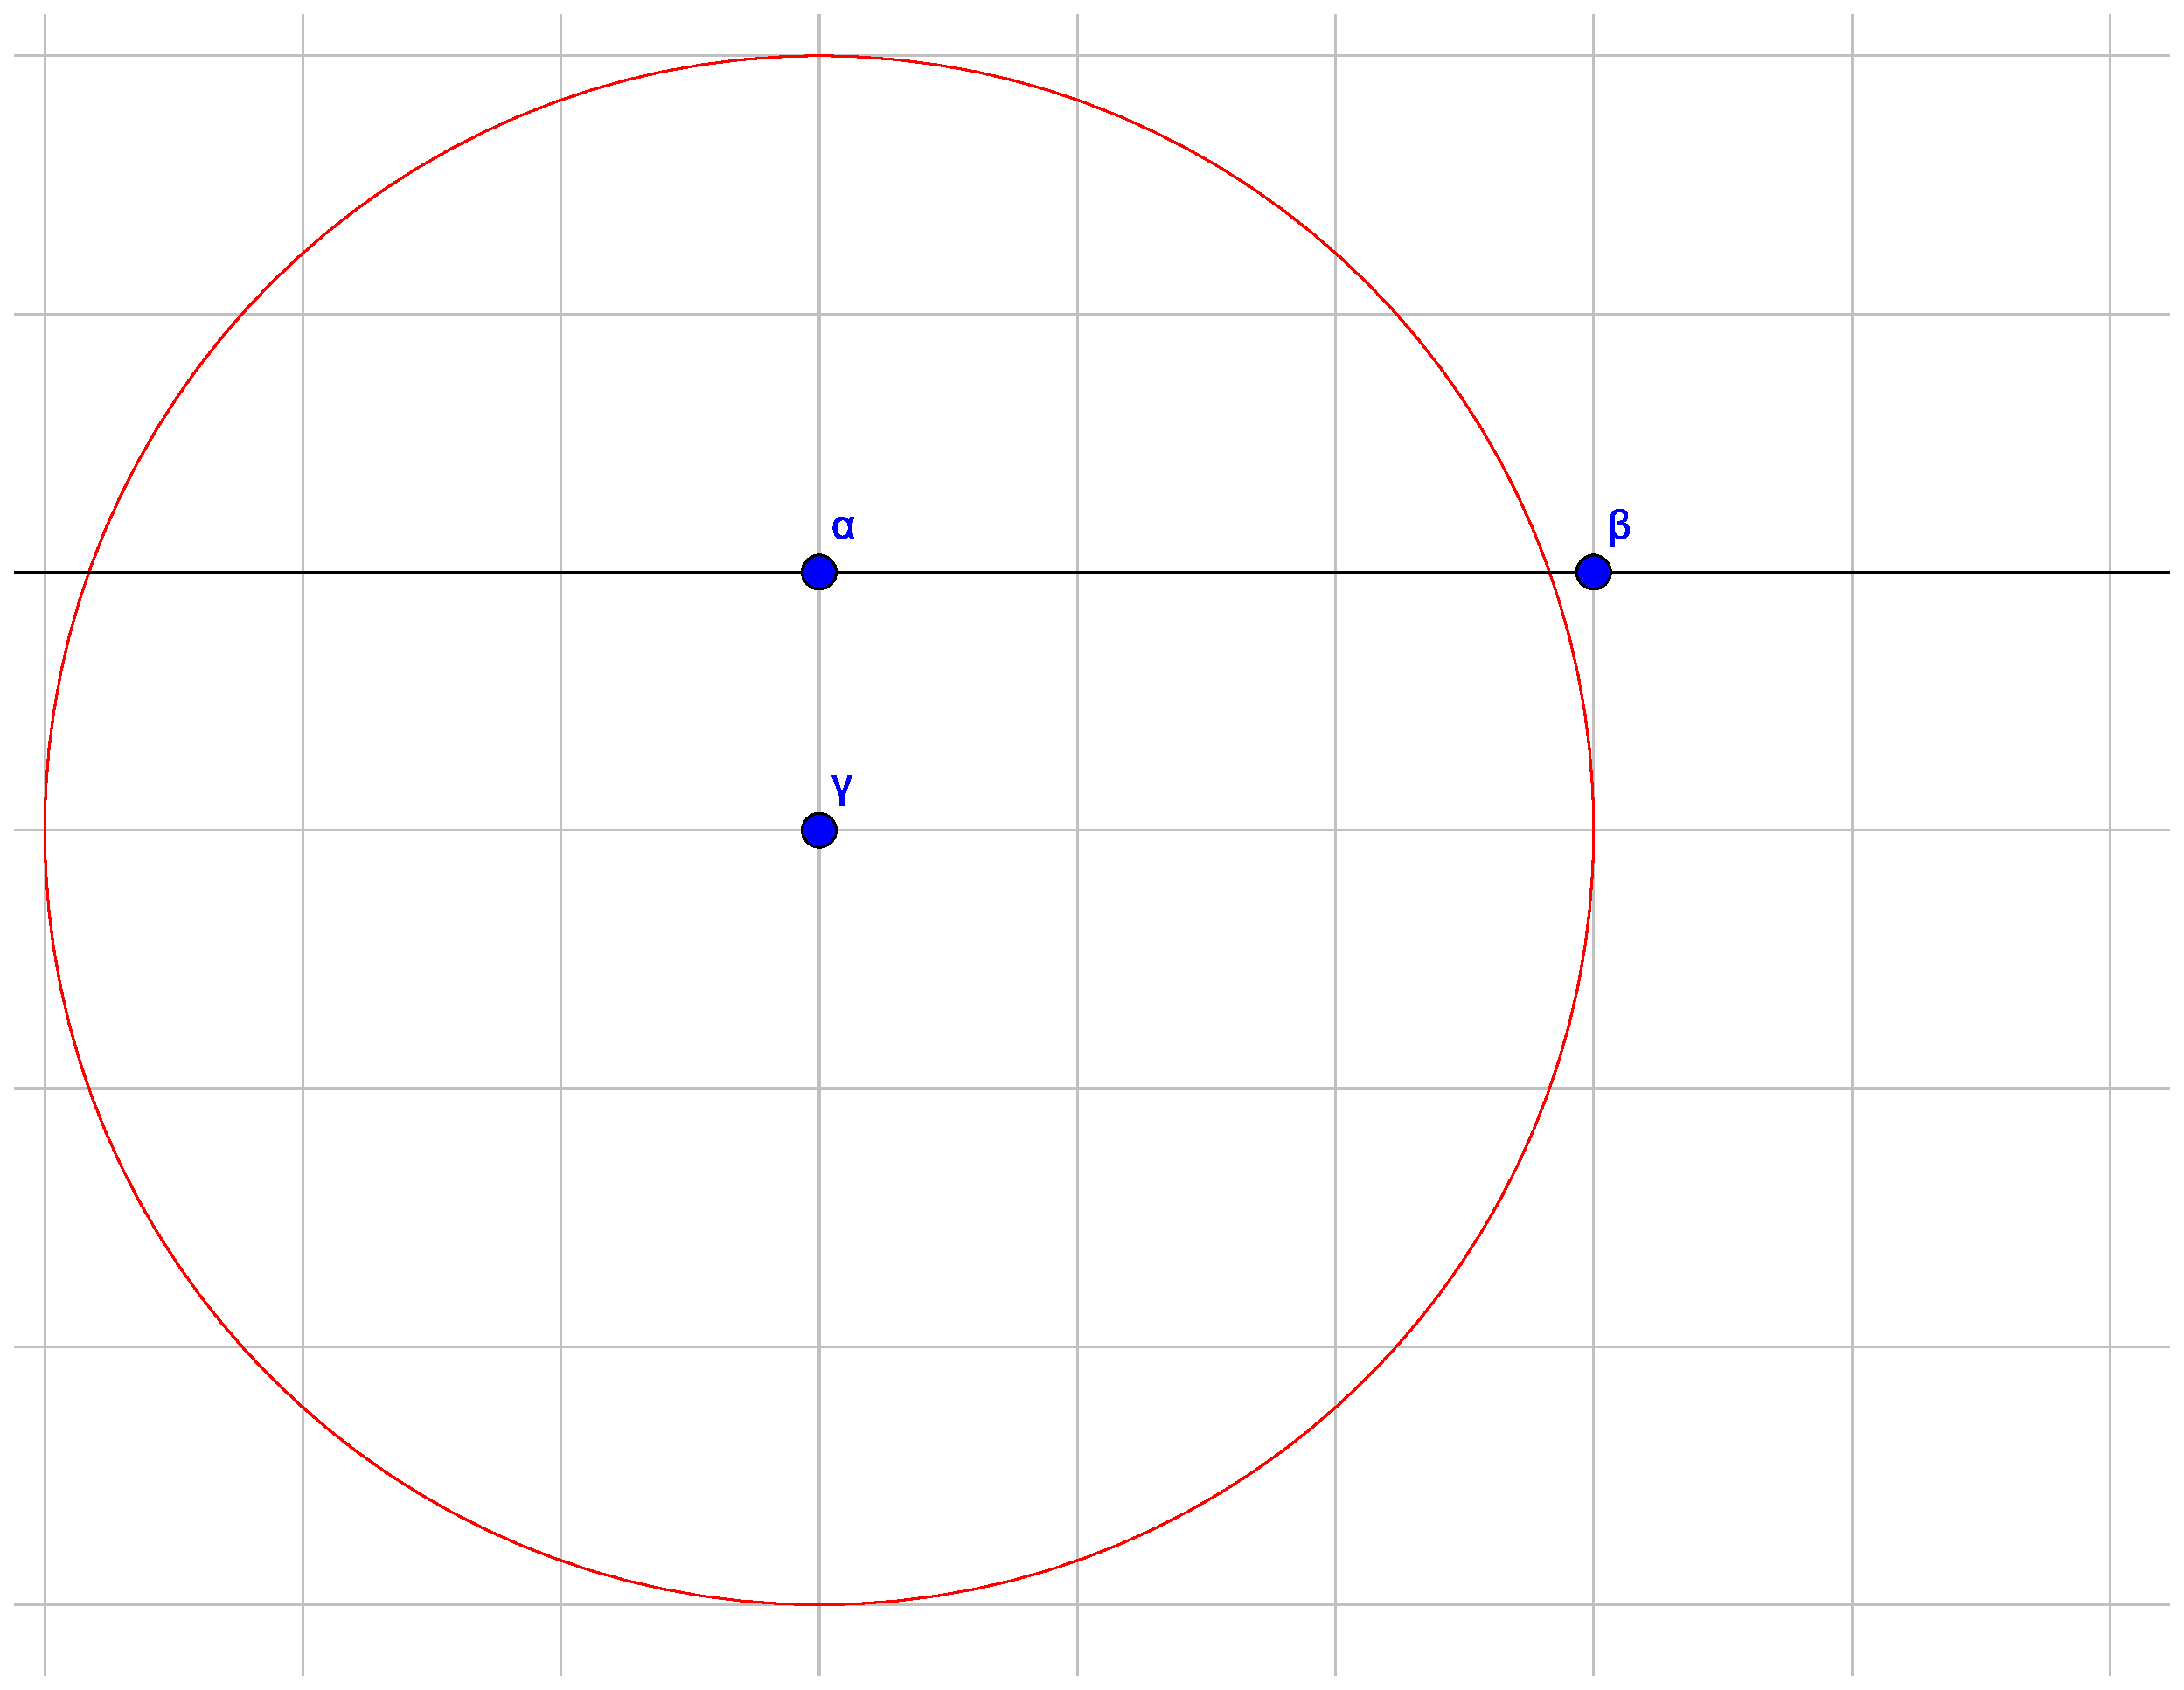
\includegraphics[scale=0.2]{C2.eps}
\label{fig:C2}
\end{figure}

\begin{block}{}
\centering
(C2)  Dla puntów $\alpha\not=\beta$ i $\gamma$ można utworzyć okrąg o środku w $\gamma$ i promieniu 
$|\alpha\beta$
\end{block}

\end{frame}


\begin{frame}{Aksjomaty}

\begin{figure}[!htb]
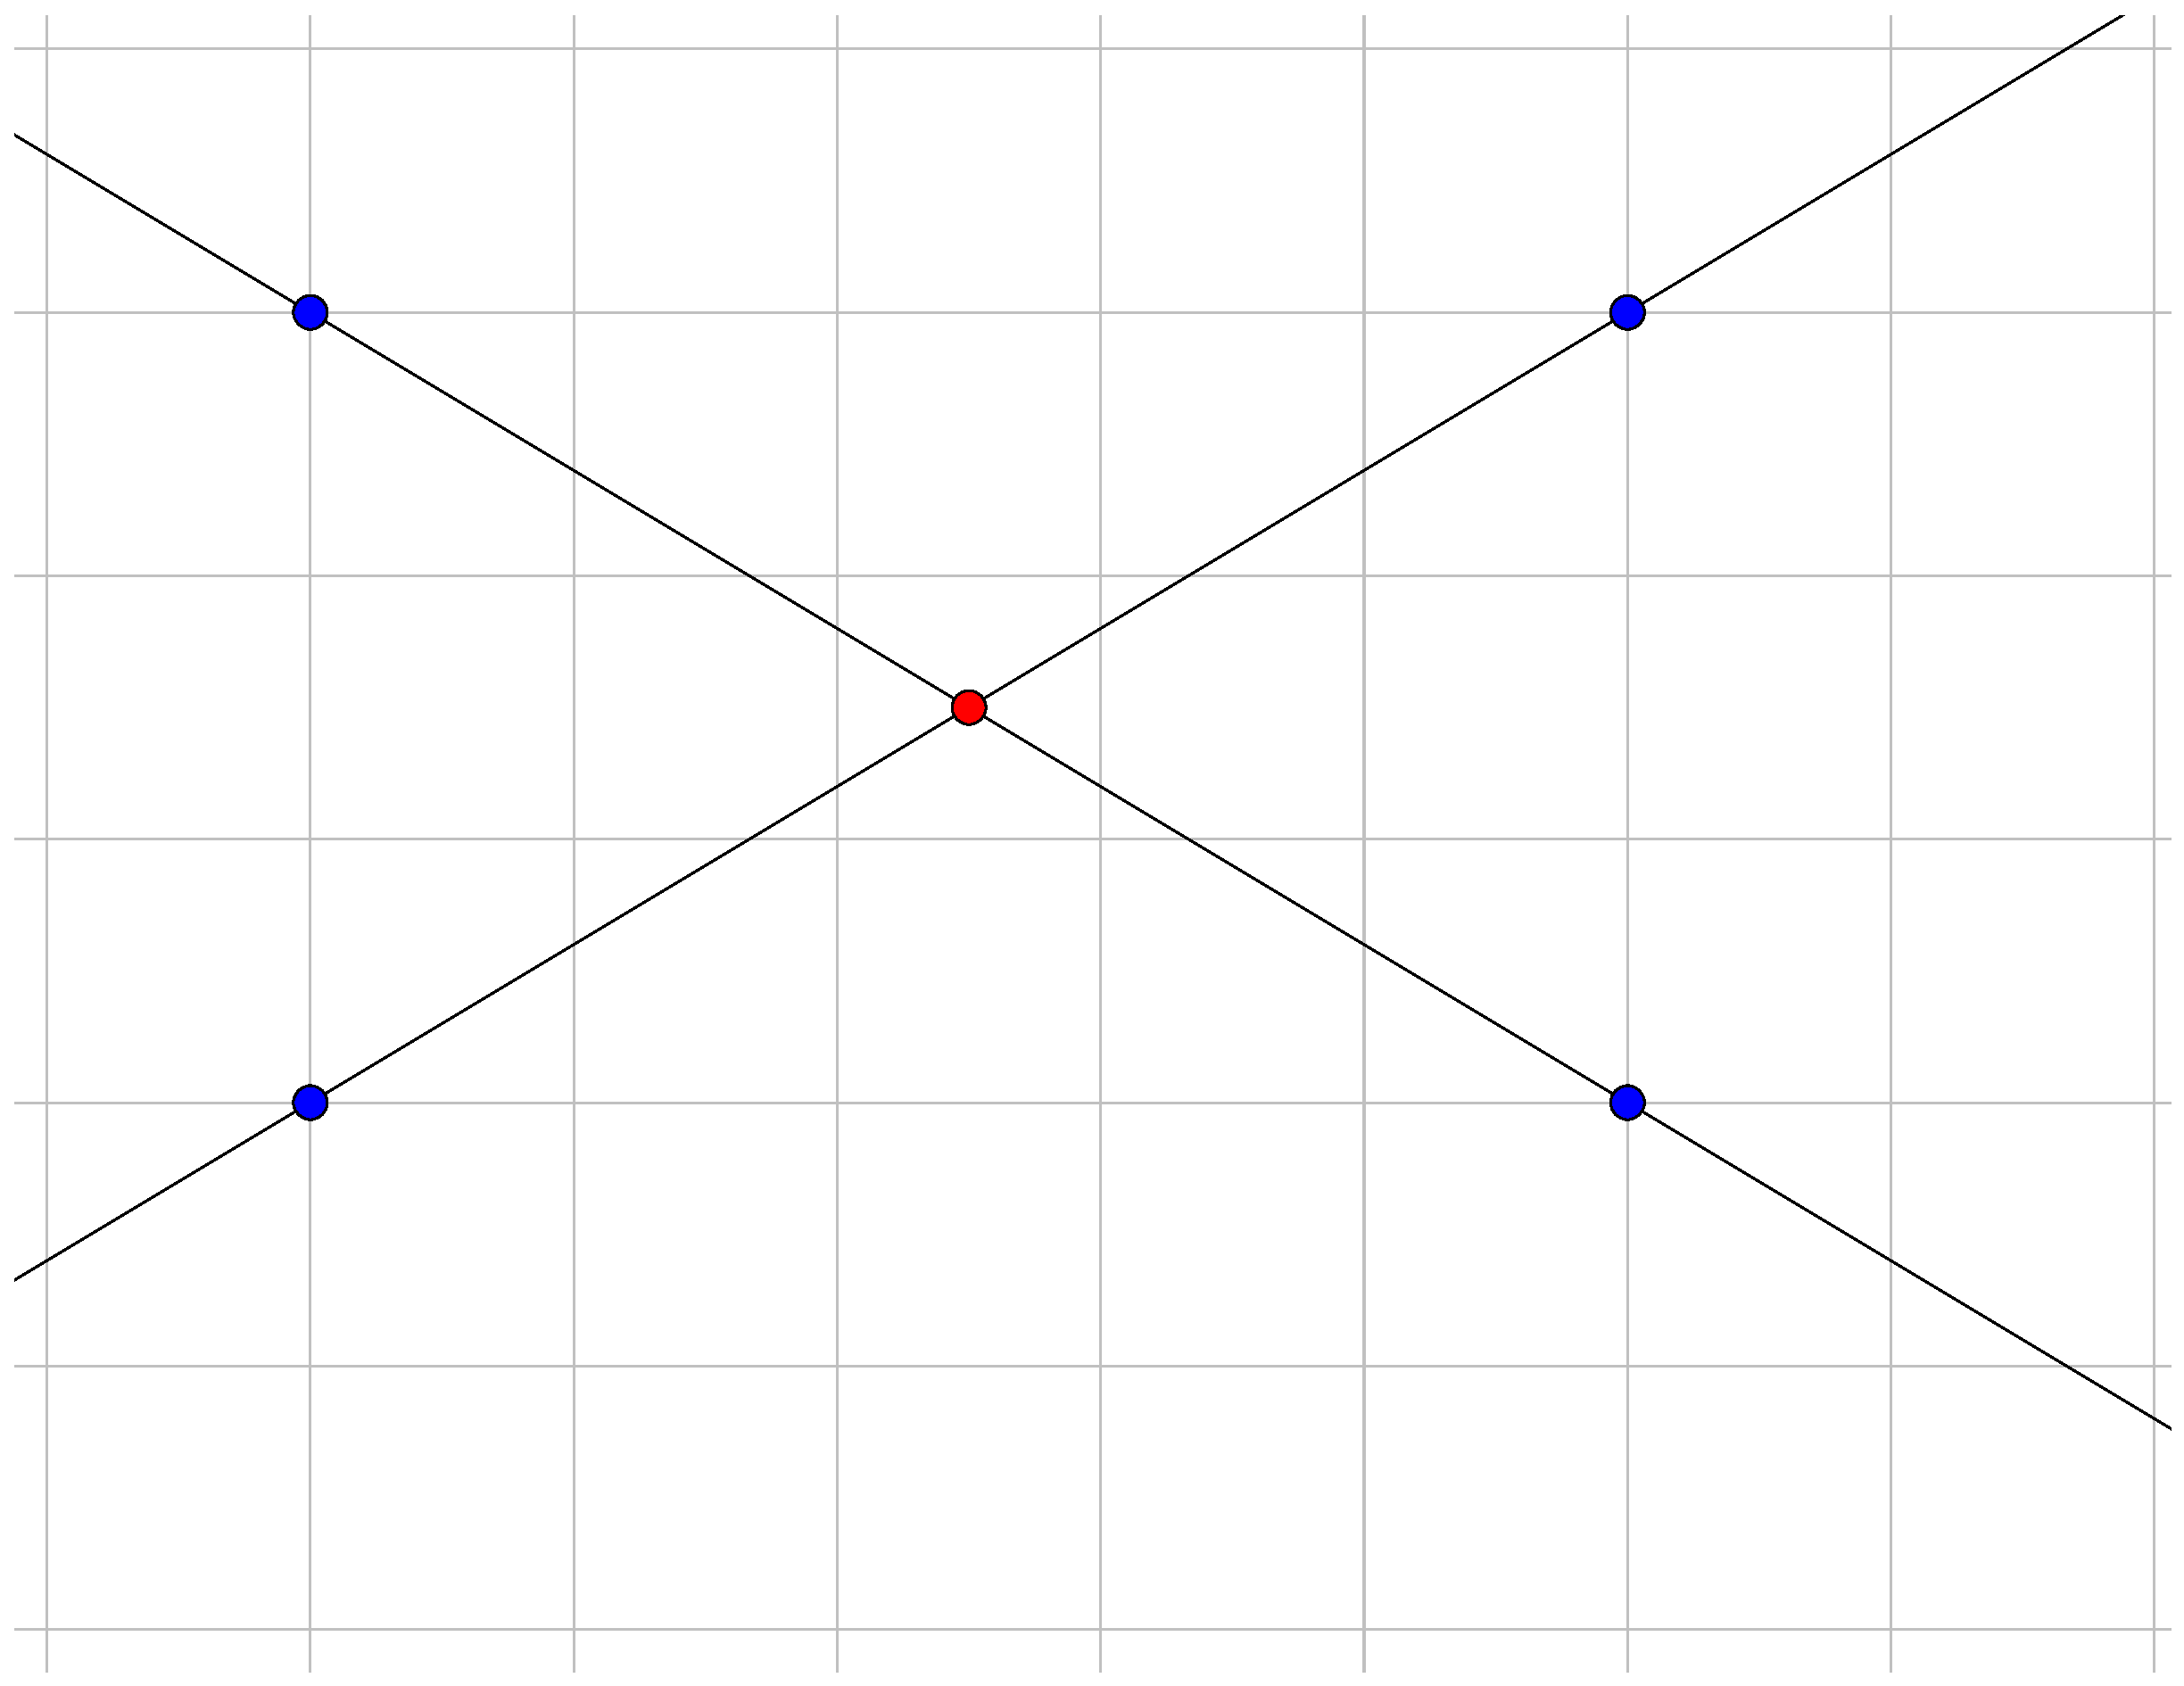
\includegraphics[scale=0.2]{P1.eps}
\label{fig:P1}
\end{figure}

\begin{block}{}
\centering
(P1)  Punkt powstaje poprzez przecięcie 2 prostych. 
\end{block}

\end{frame}


\begin{frame}{Aksjomaty}

\begin{figure}[!htb]
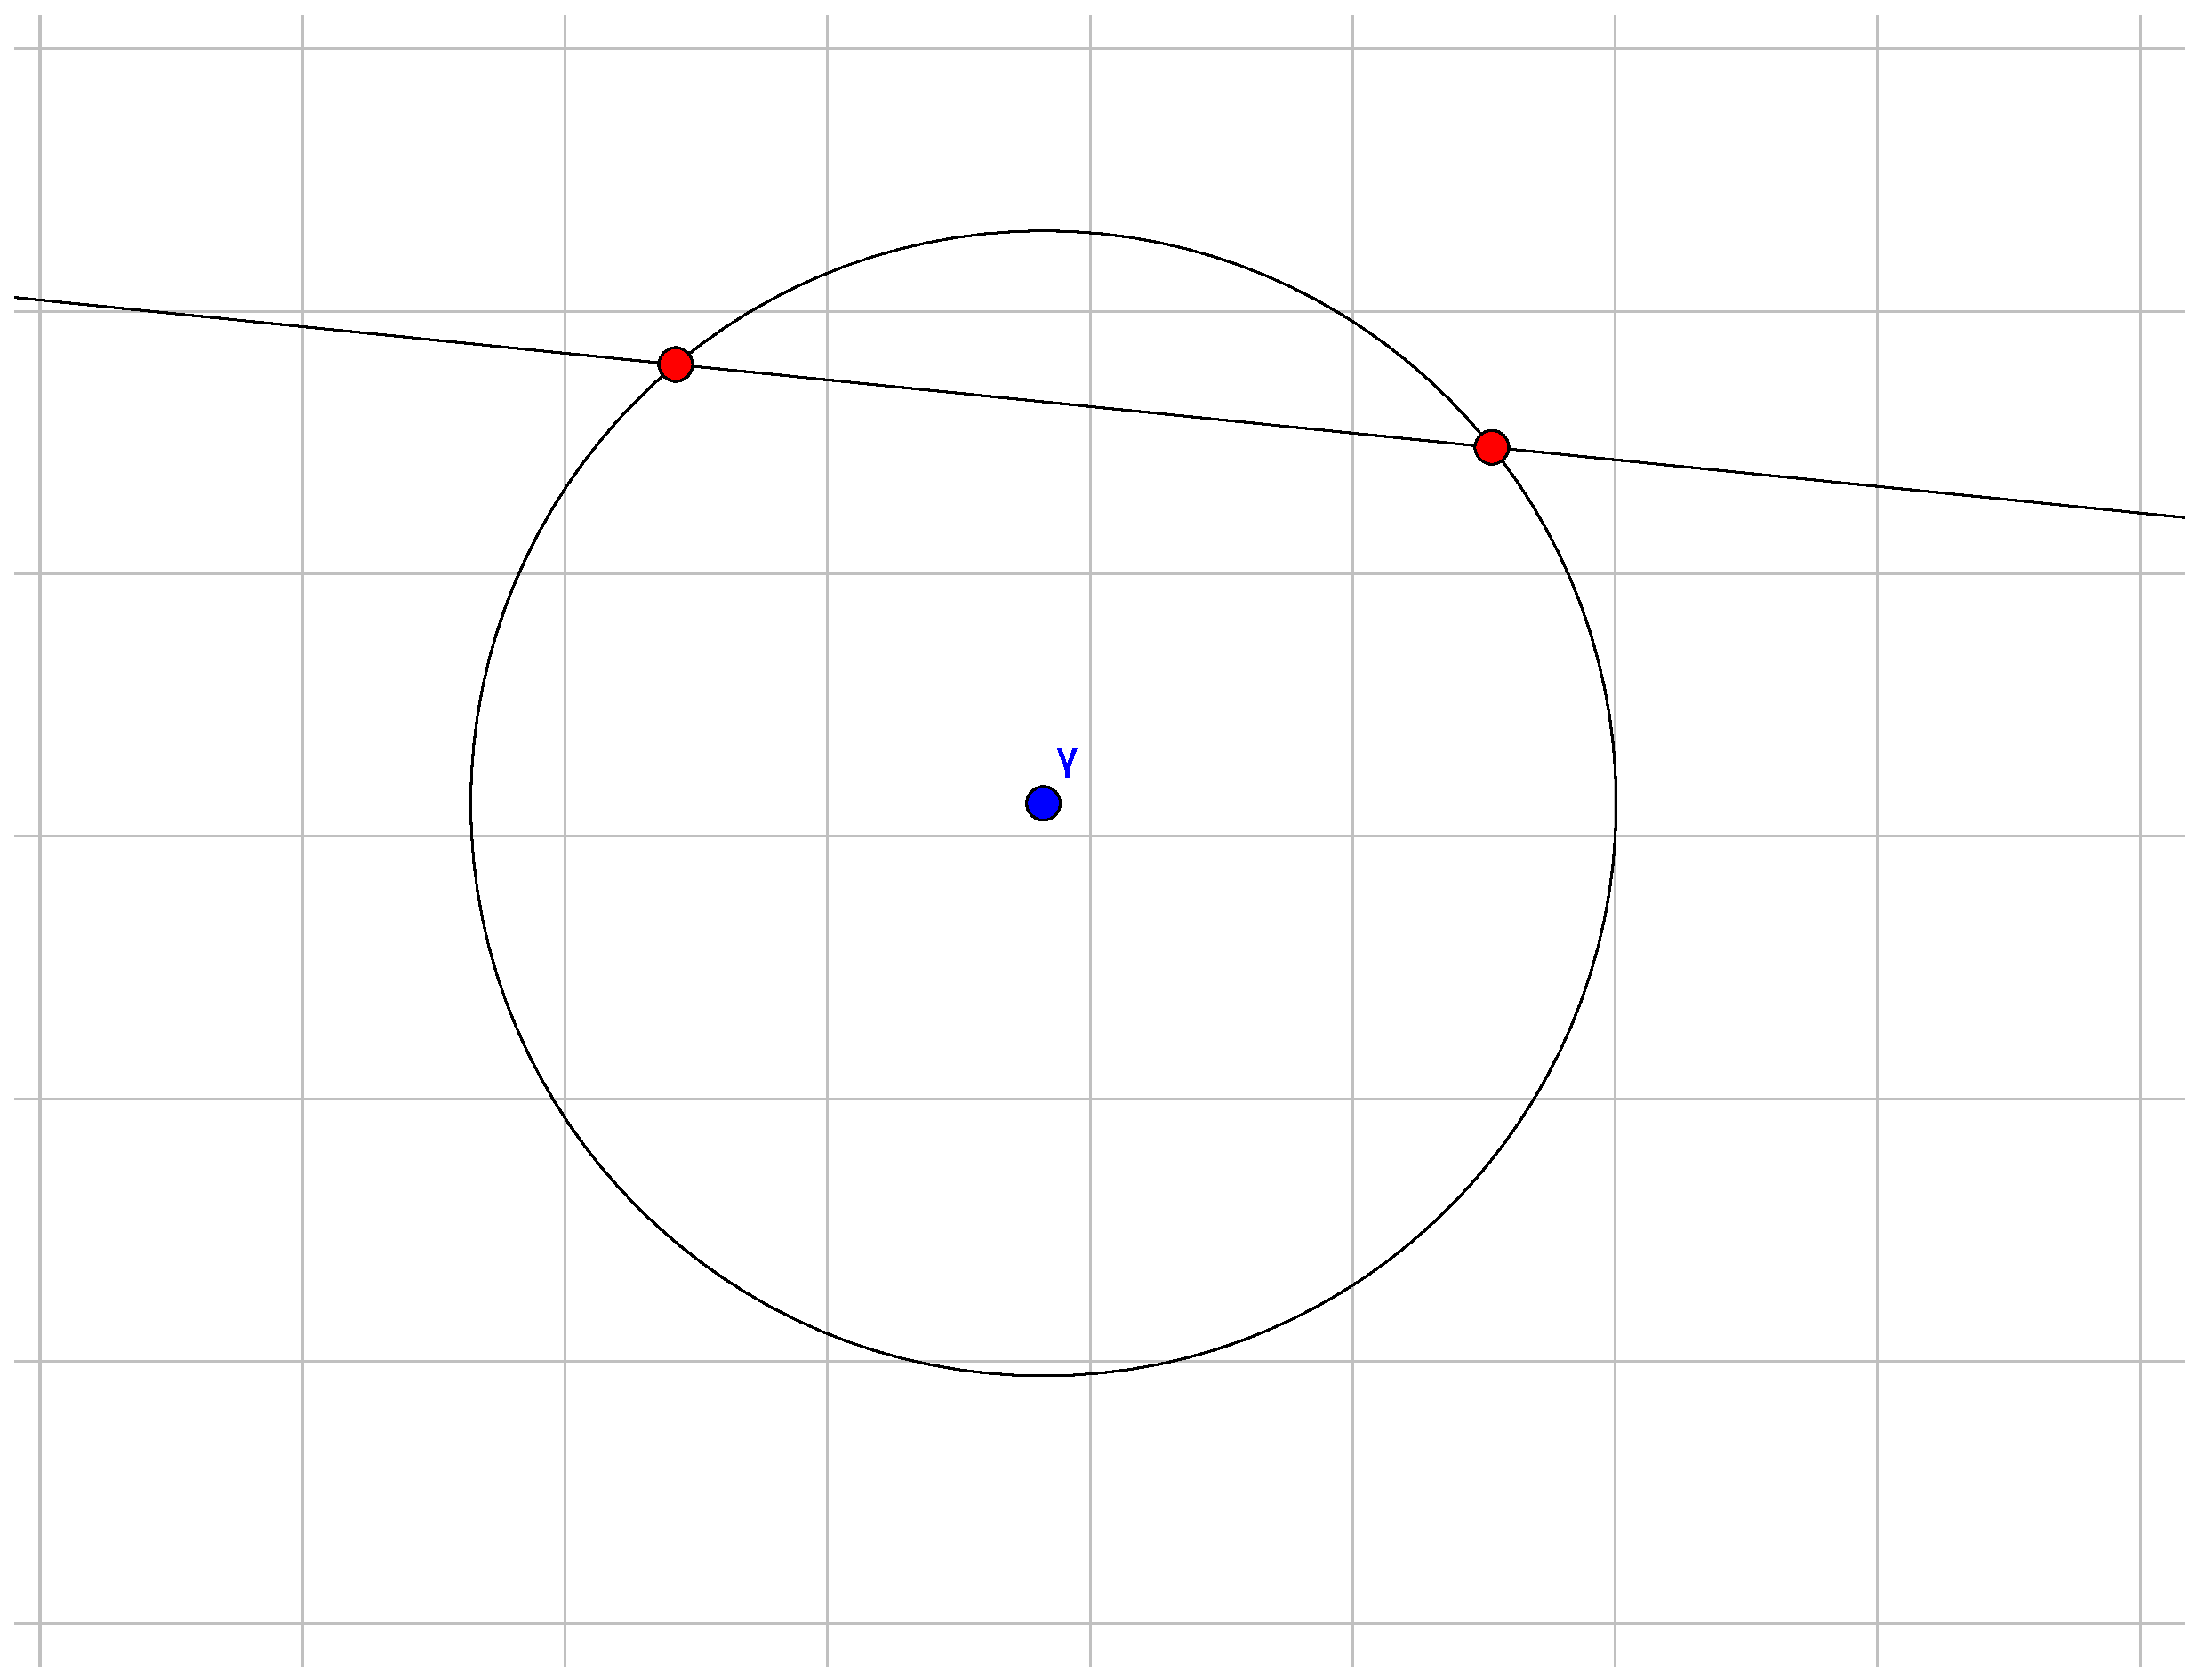
\includegraphics[scale=0.2]{P2.eps}
\label{fig:P2}
\end{figure}

\begin{block}{}
\centering
(P2)  Punkt powstaje przez przecięcie prostej i okręgu.
\end{block}

\end{frame}


\begin{frame}{Aksjomaty}

\begin{figure}[!htb]
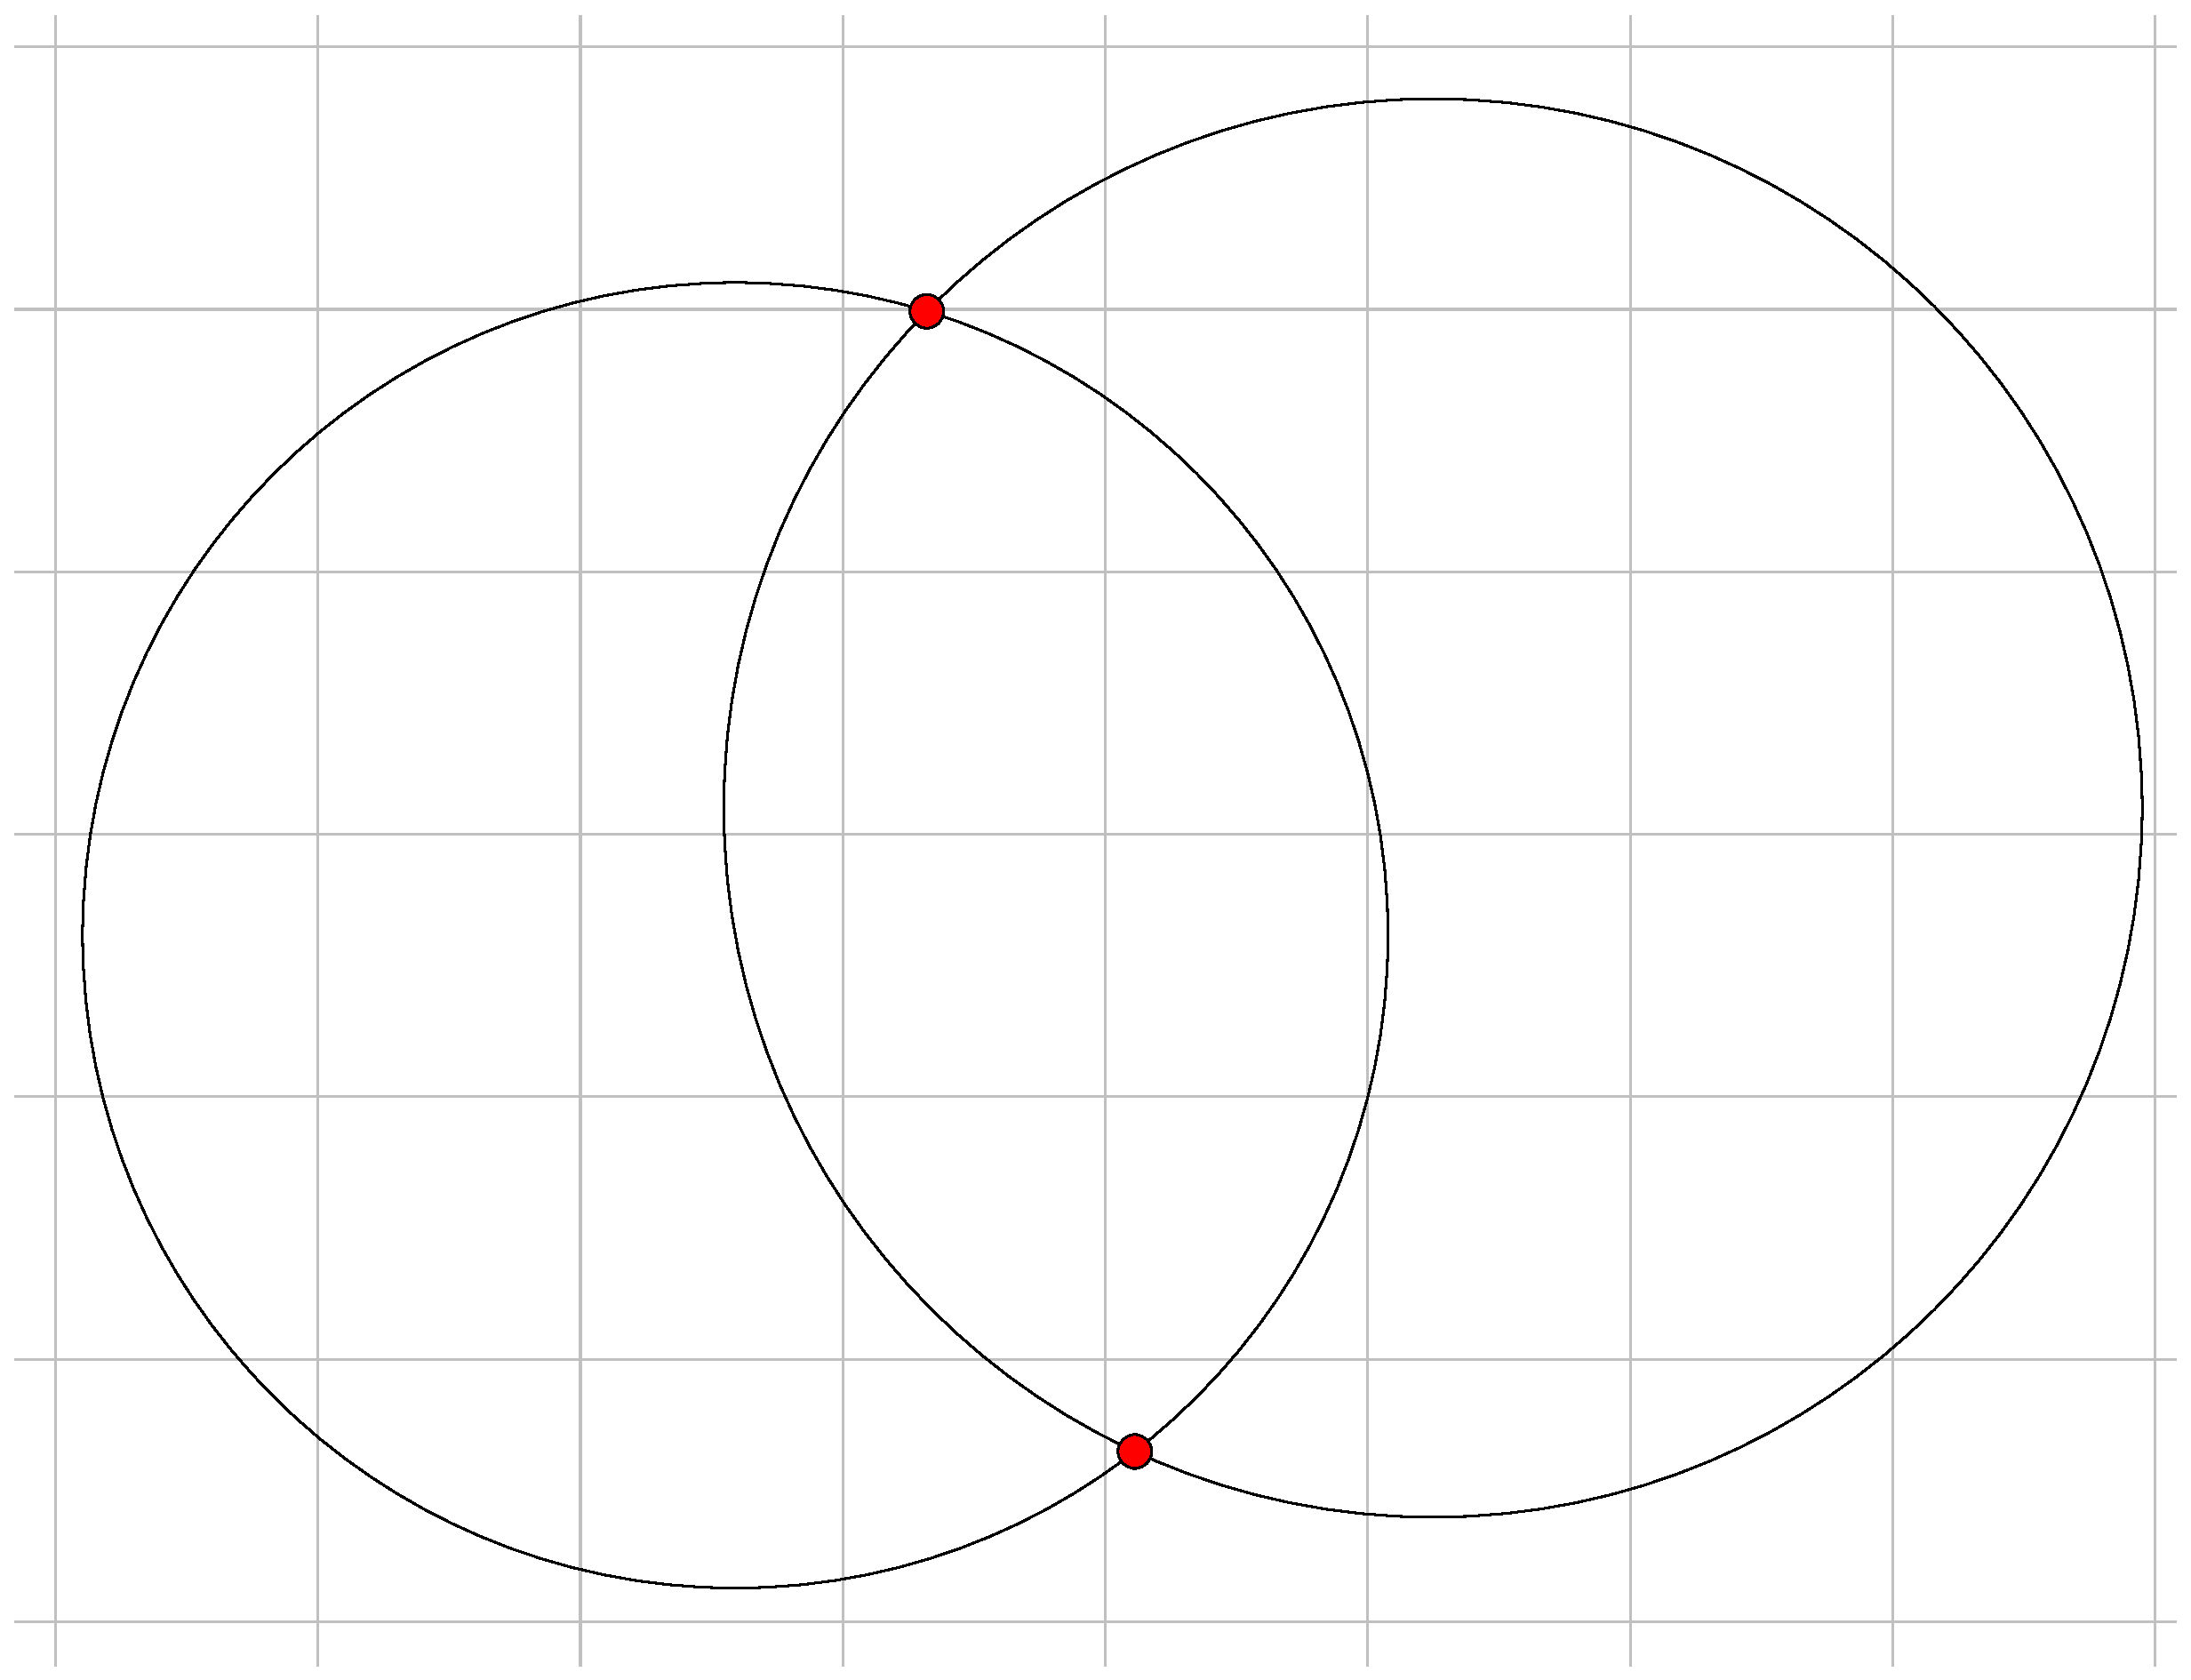
\includegraphics[scale=0.2]{P3.eps}
\label{fig:digraph}
\end{figure}

\begin{block}{}
\centering
(P3)  Punkt powstaje przez przecięcie dwóch okręgów.
\end{block}

\end{frame}

\section{Liczby Konstruowalne}


\begin{frame}{Liczby Konstruowalne}
\begin{definicja}
Liczba zespololona jest konstruowalna. 
\end{definicja}
\end{frame}

\begin{frame}{Liczby Konstruowalne}
\begin{przyklad}
Liczby naturalne
\begin{figure}[!htb]
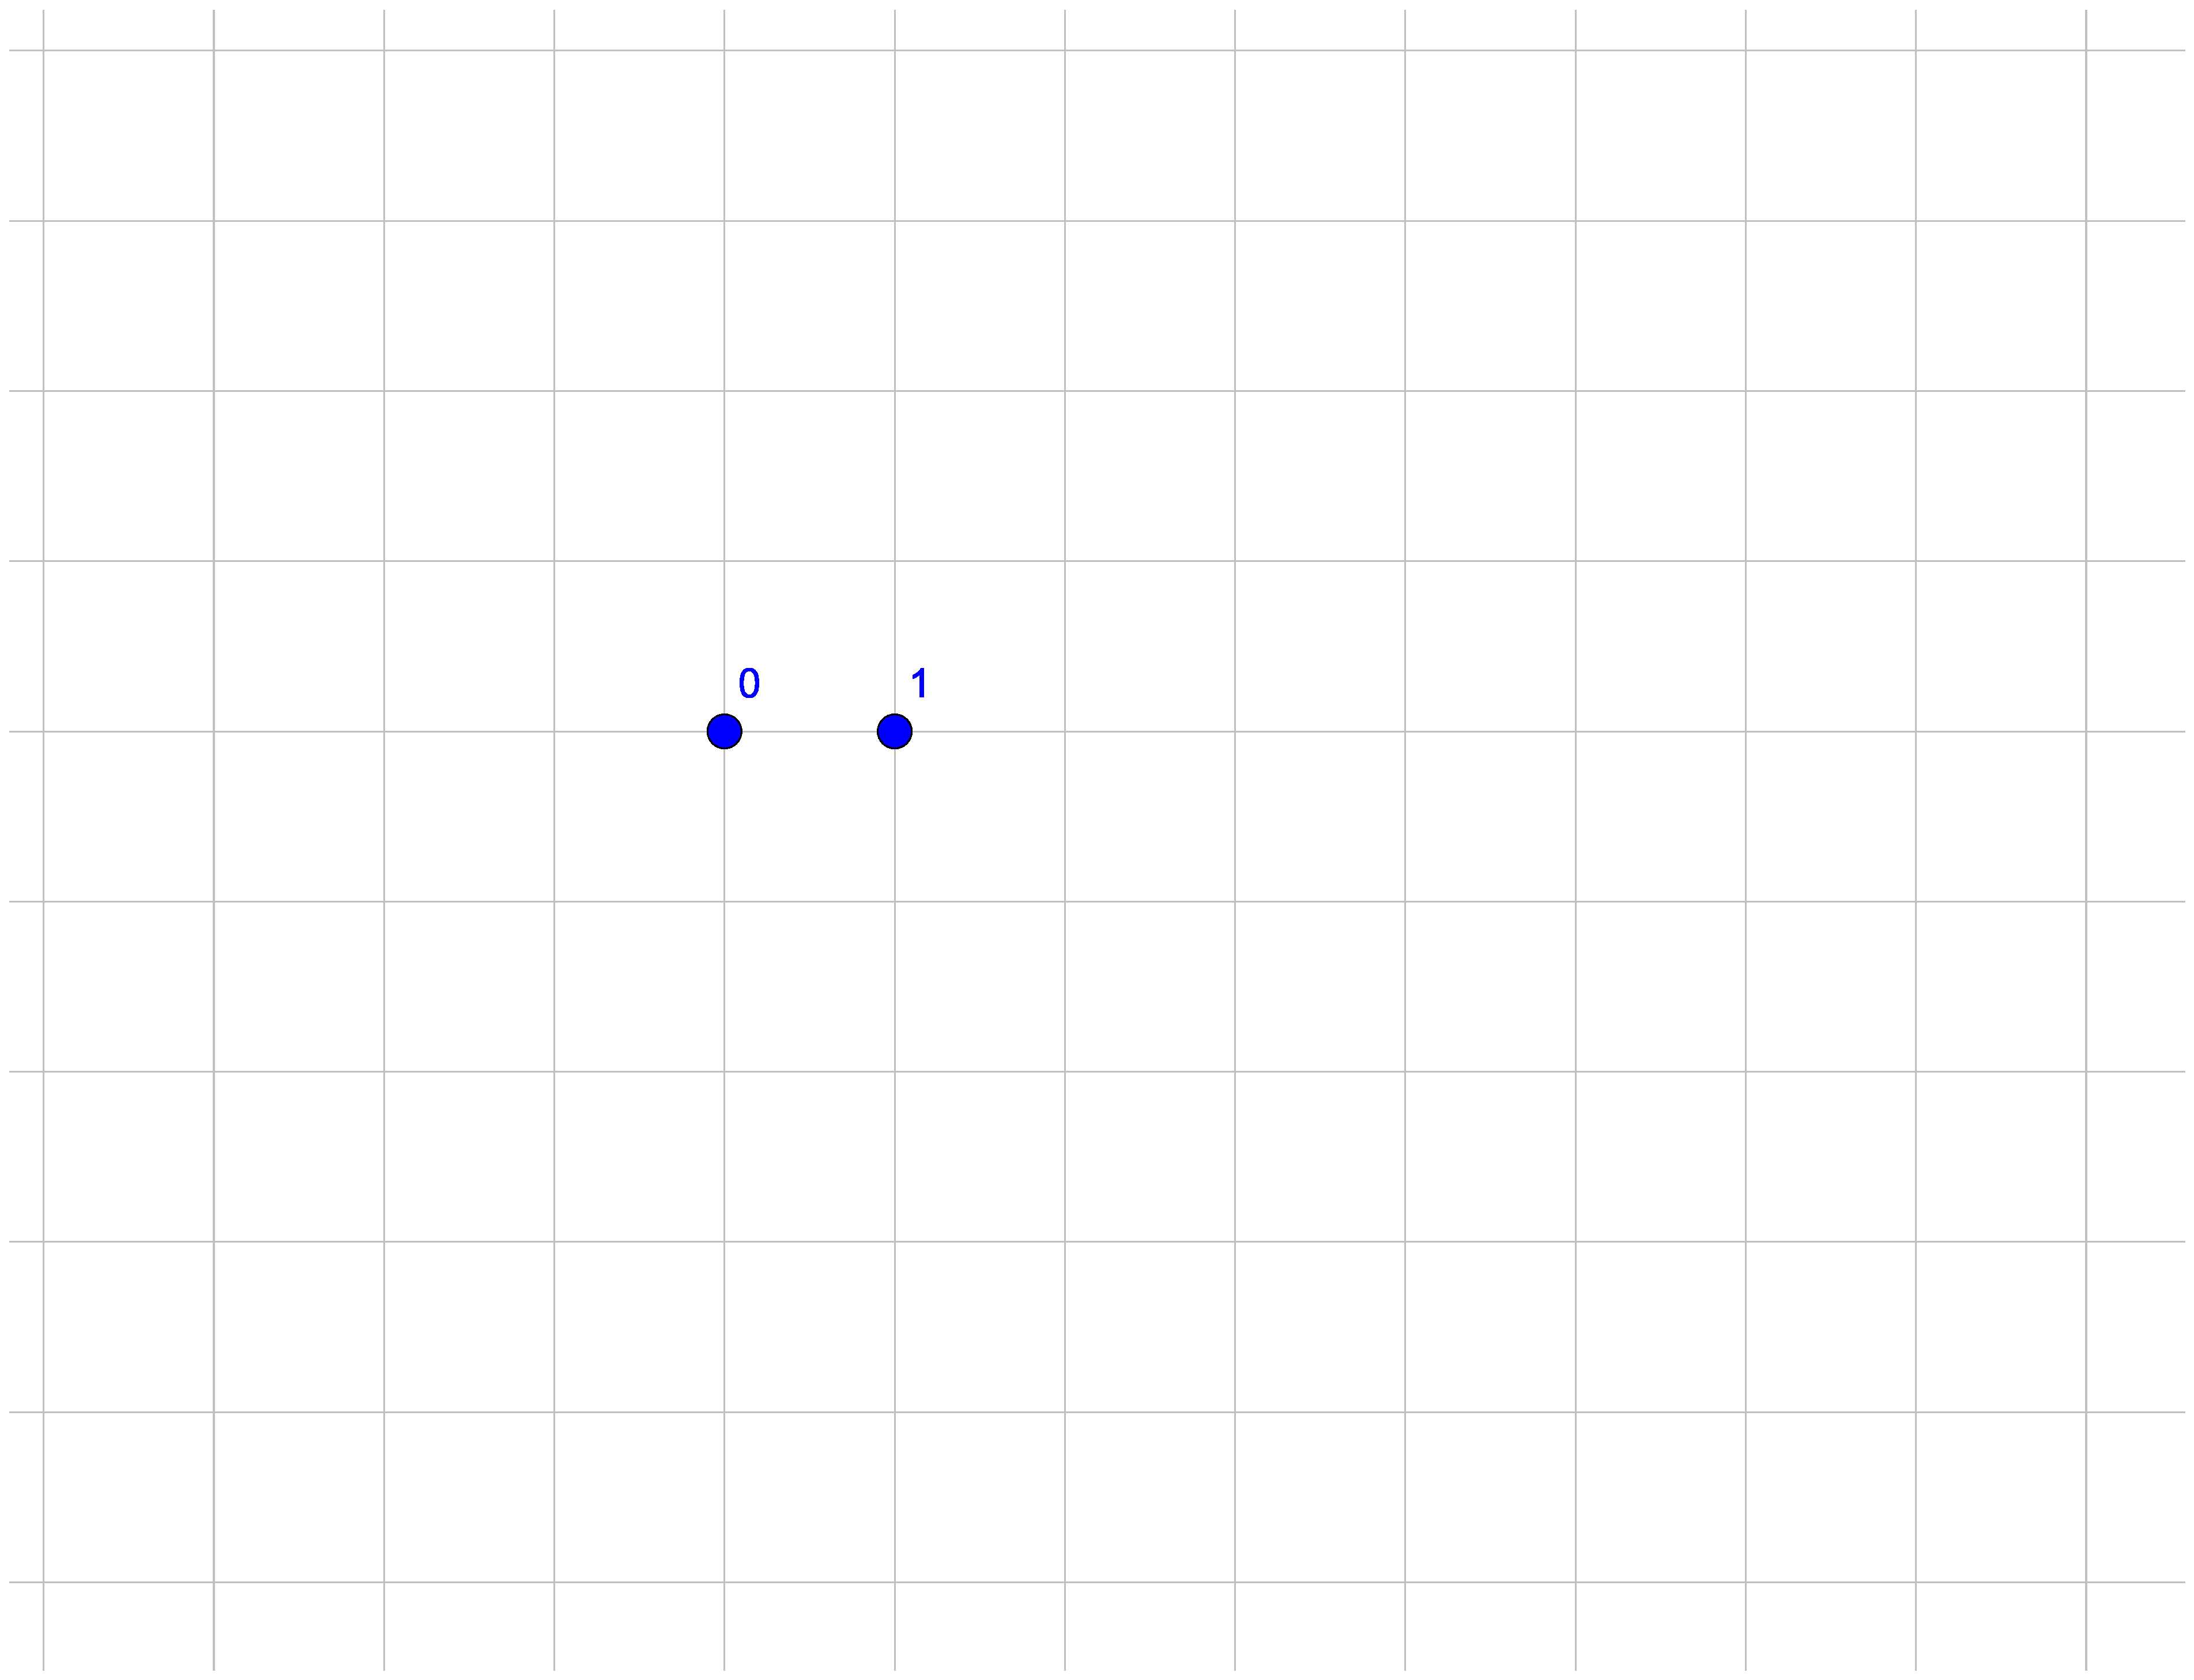
\includegraphics[scale=0.1]{ex1.eps}
\label{fig:ex1}
\end{figure}
\end{przyklad}
\end{frame}

\begin{frame}{Liczby Konstruowalne}
\begin{przyklad}
Liczby naturalne
\begin{figure}[!htb]
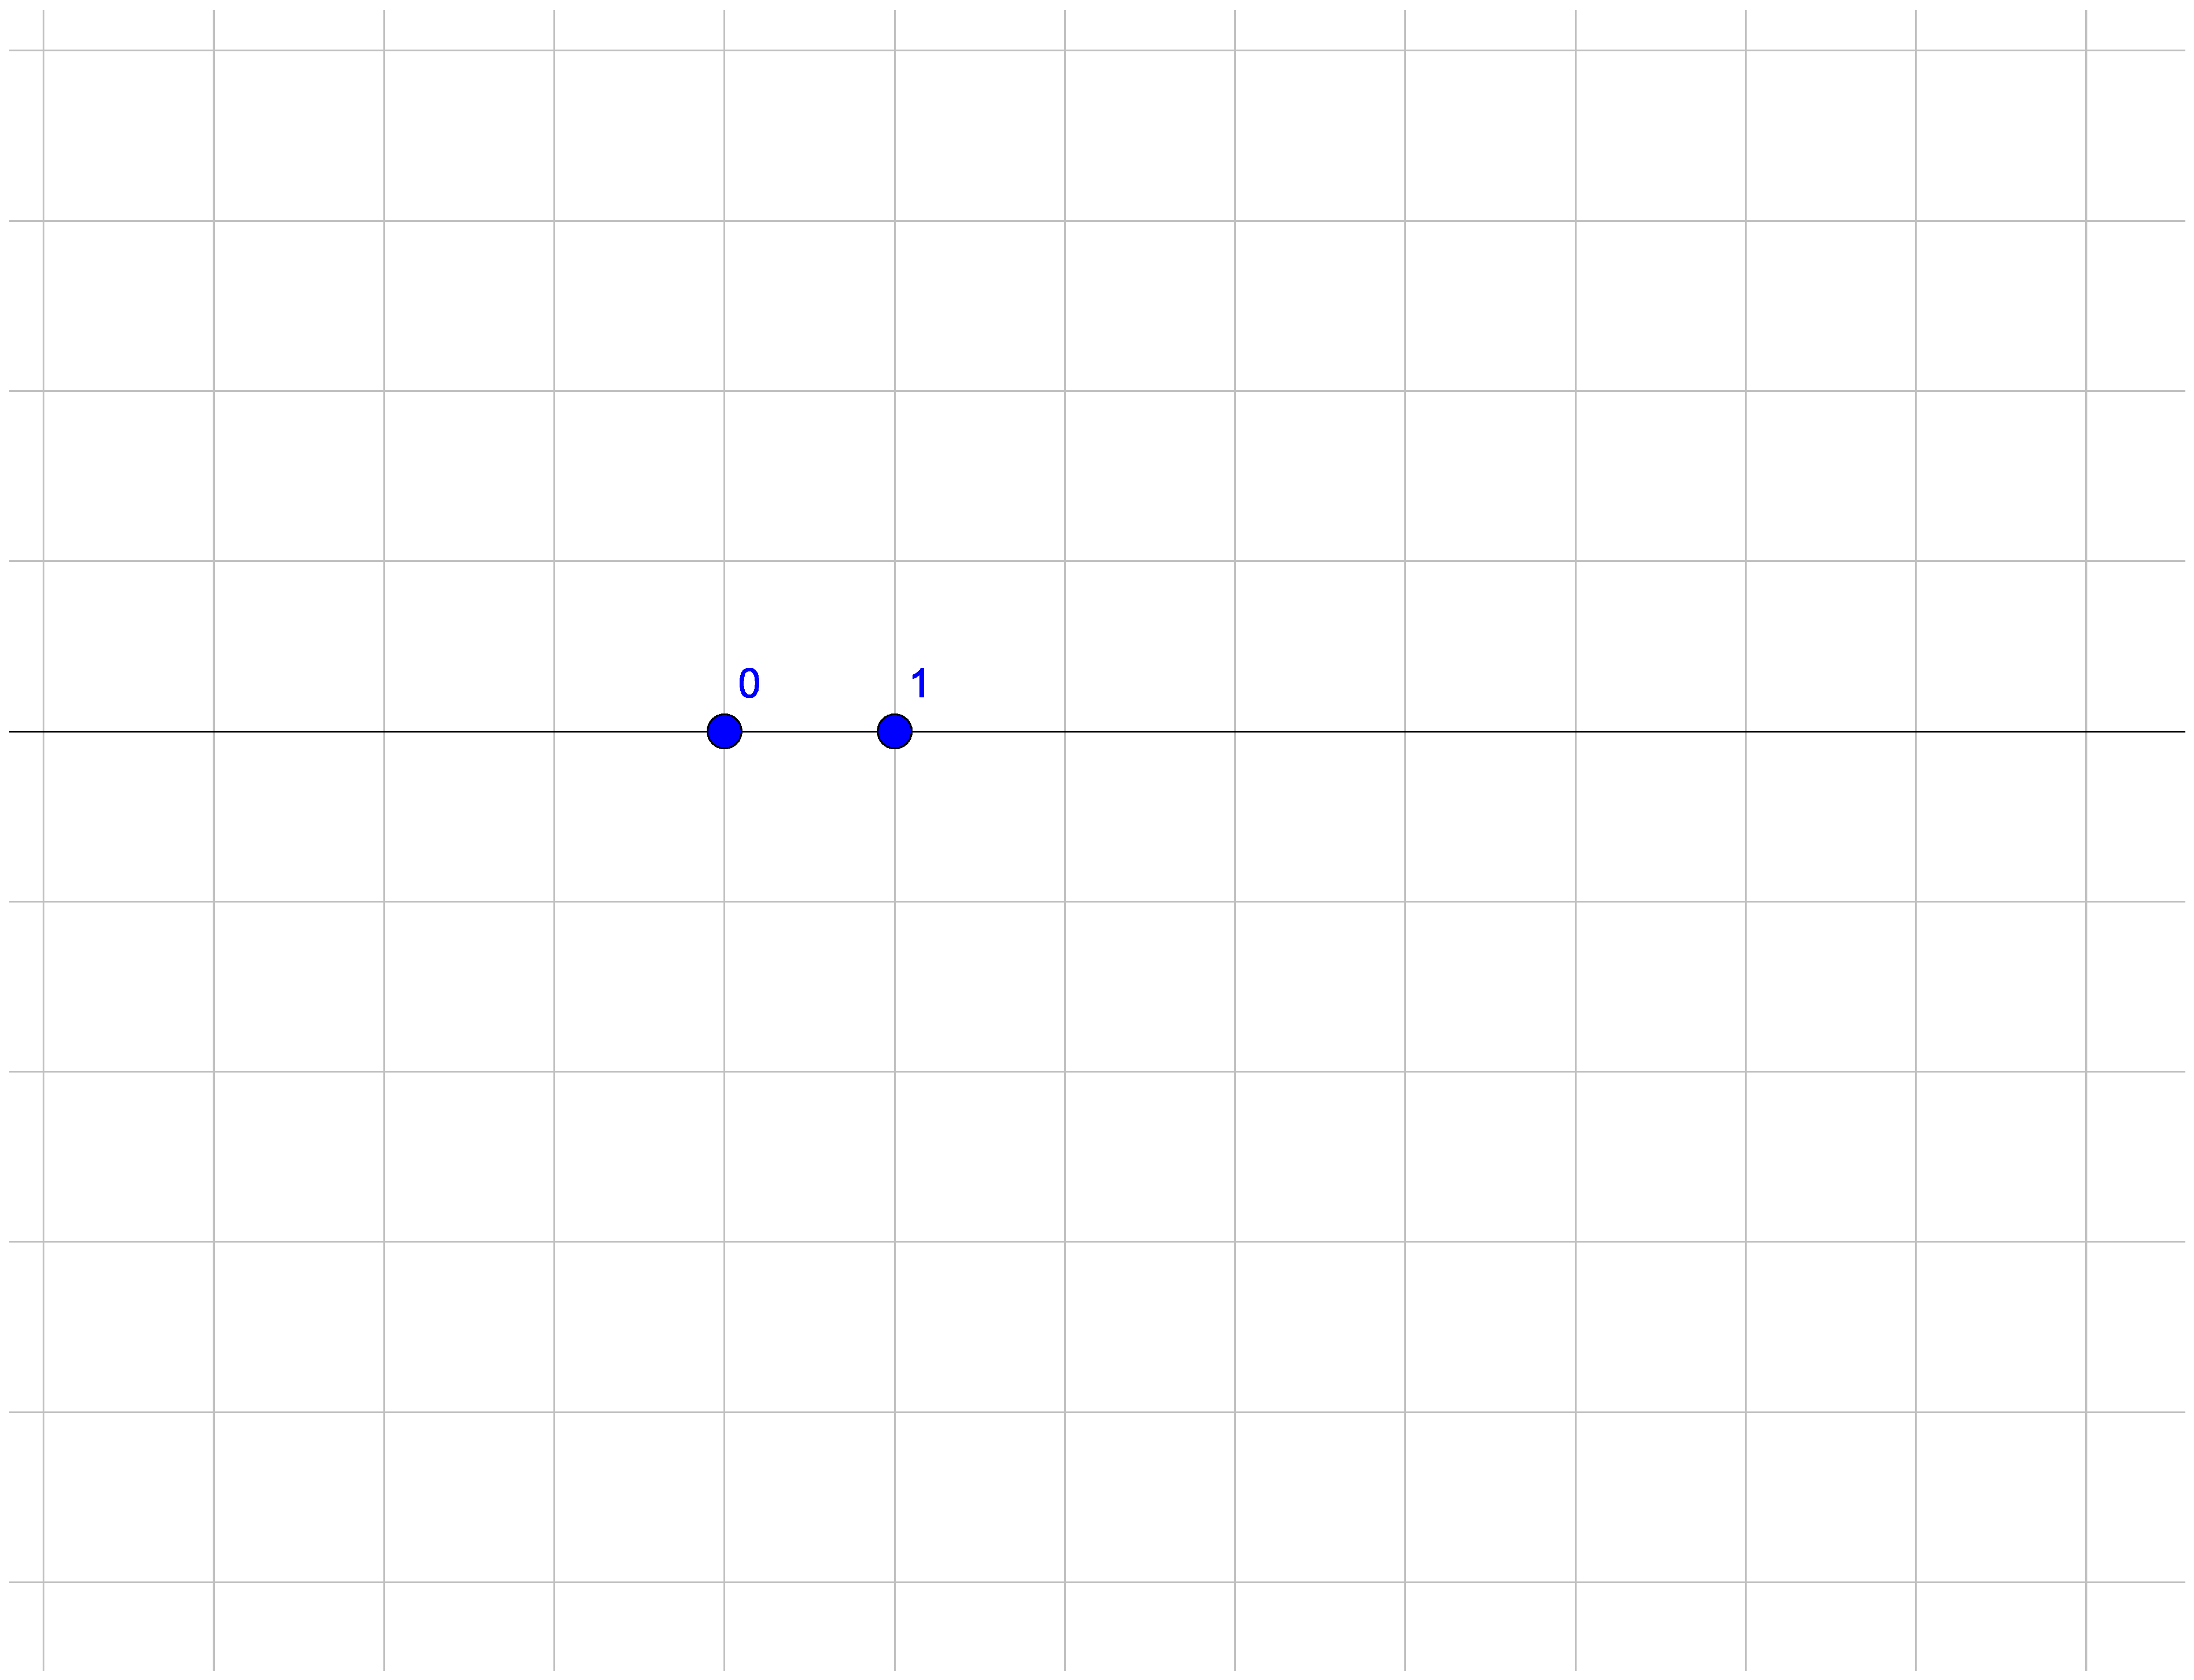
\includegraphics[scale=0.1]{ex2.eps}
\label{fig:ex2}
\end{figure}
\end{przyklad}
\end{frame}

\begin{frame}{Liczby Konstruowalne}
\begin{przyklad}
Liczby naturalne
\begin{figure}[!htb]
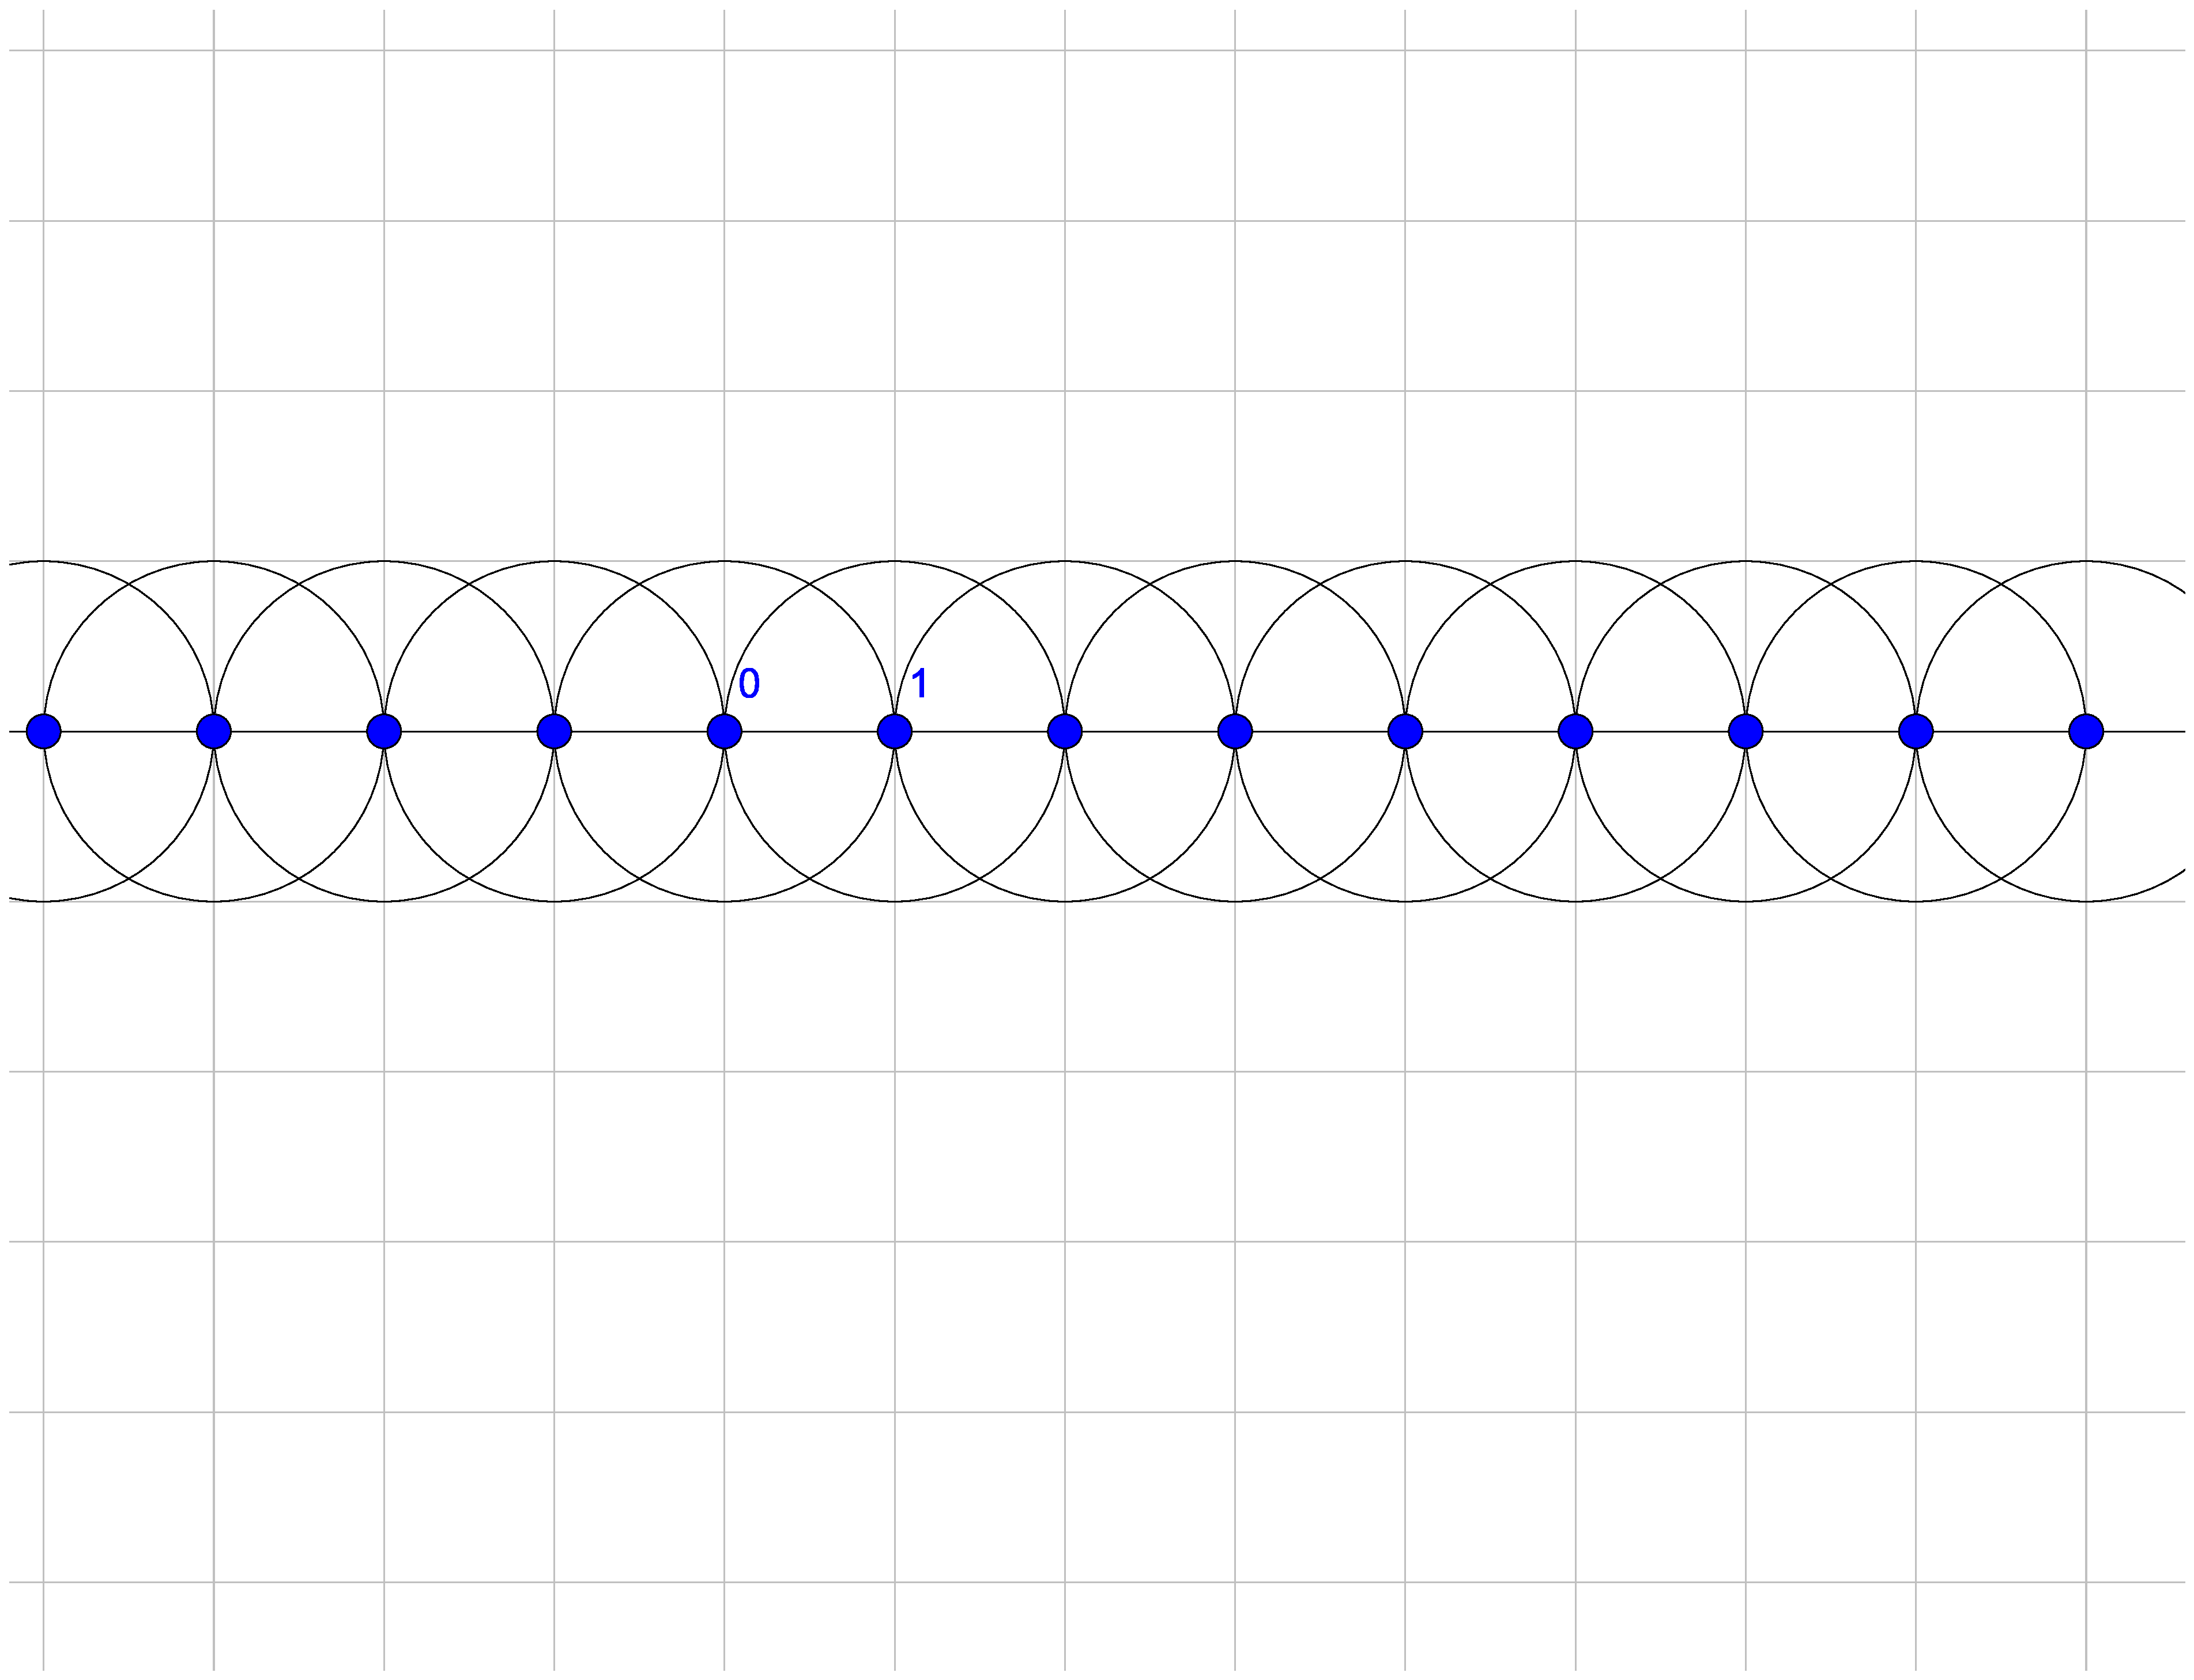
\includegraphics[scale=0.1]{ex3.eps}
\label{fig:ex3}
\end{figure}
\end{przyklad}
\end{frame}

\begin{frame}{Liczby Konstruowalne}
\begin{przyklad}
Liczby urojone całkowite
\begin{figure}[!htb]
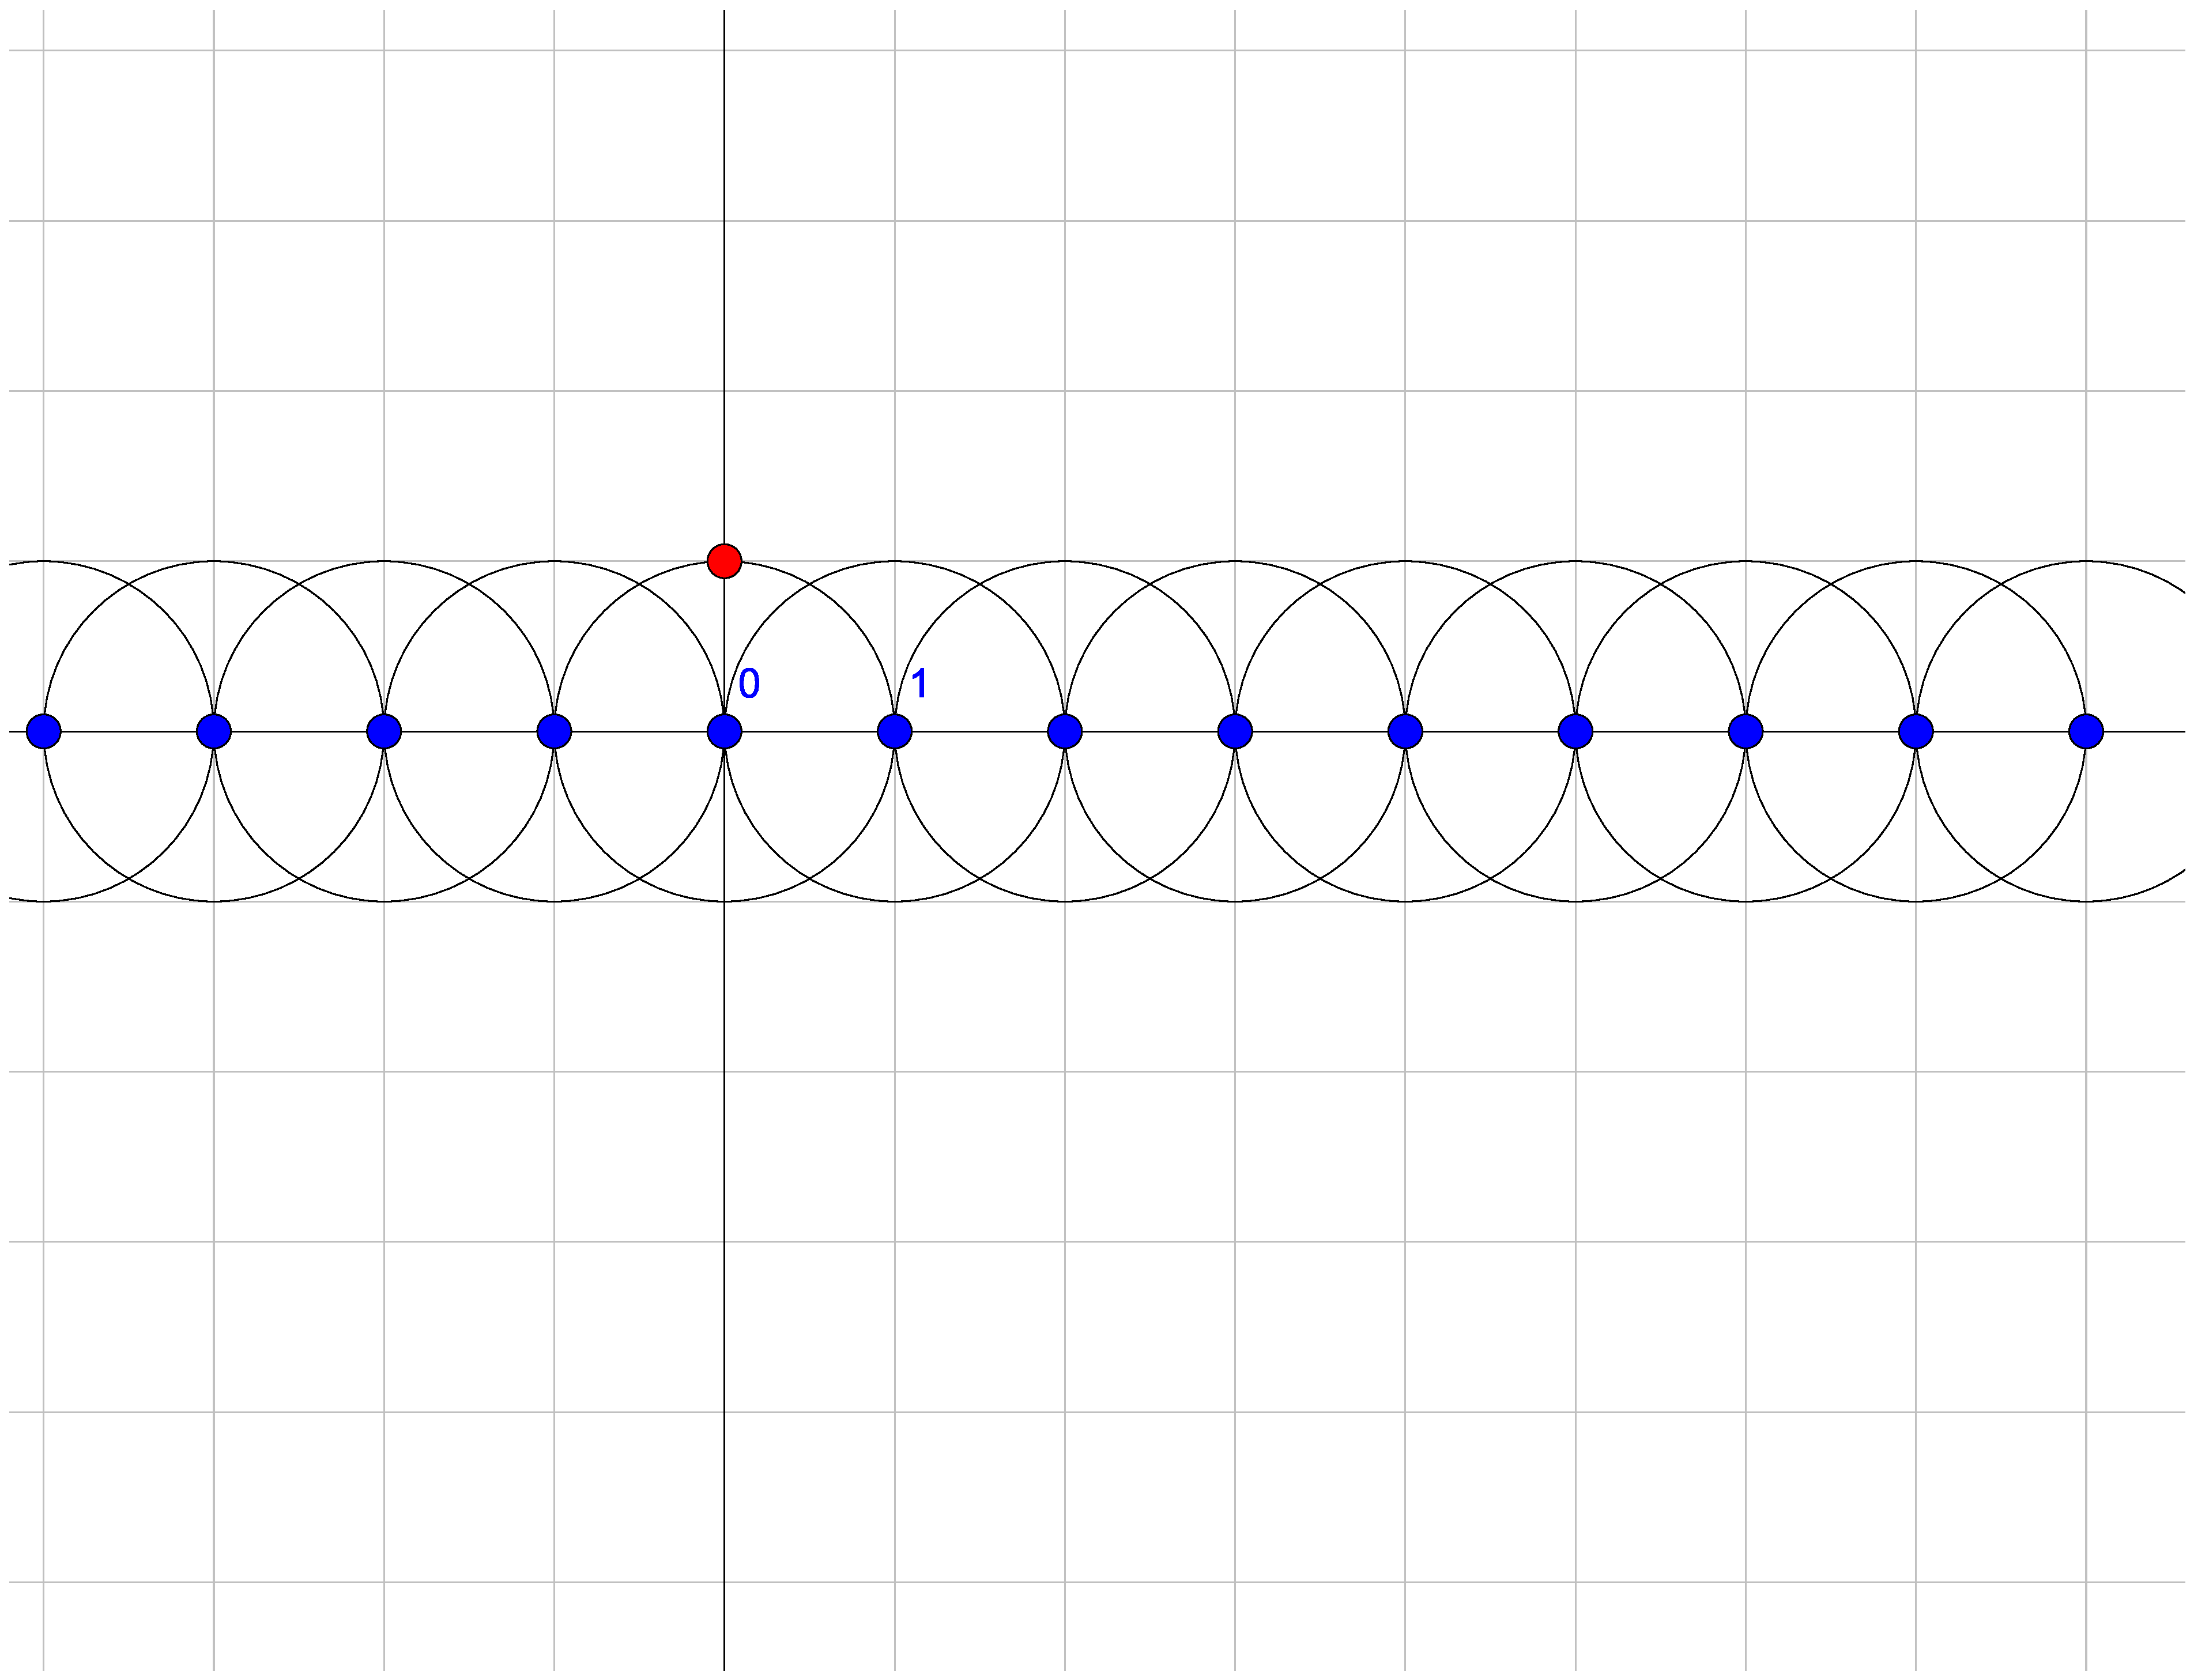
\includegraphics[scale=0.1]{ex4.eps}
\label{fig:ex4}
\end{figure}
\end{przyklad}
\end{frame}

\begin{frame}{Liczby Konstruowalne}
\begin{twierdzenie}
Niech $\mathcal{C}=\{\alpha\in\mathbb{C}\ |\ \alpha\ jest\ konstuowalne\}$ $\mathcal{C}$ jest podciałem 	$\mathbb{C}$ Ponadto: 
\begin{enumerate}[label=(\alph*)]
\item Niech $\alpha = a + bi\in\mathcal{C}$, gdzie $a,b\in\mathbb{R}$, to $a,b\in\mathcal{C}$.
\item Jeżeli $\alpha \in \mathcal{C}$, to $\sqrt{\alpha}\in\mathcal{C}$
\end{enumerate}
\end{twierdzenie}
\end{frame}

\begin{frame}{Liczby Konstruowalne}
\begin{figure}[!htb]
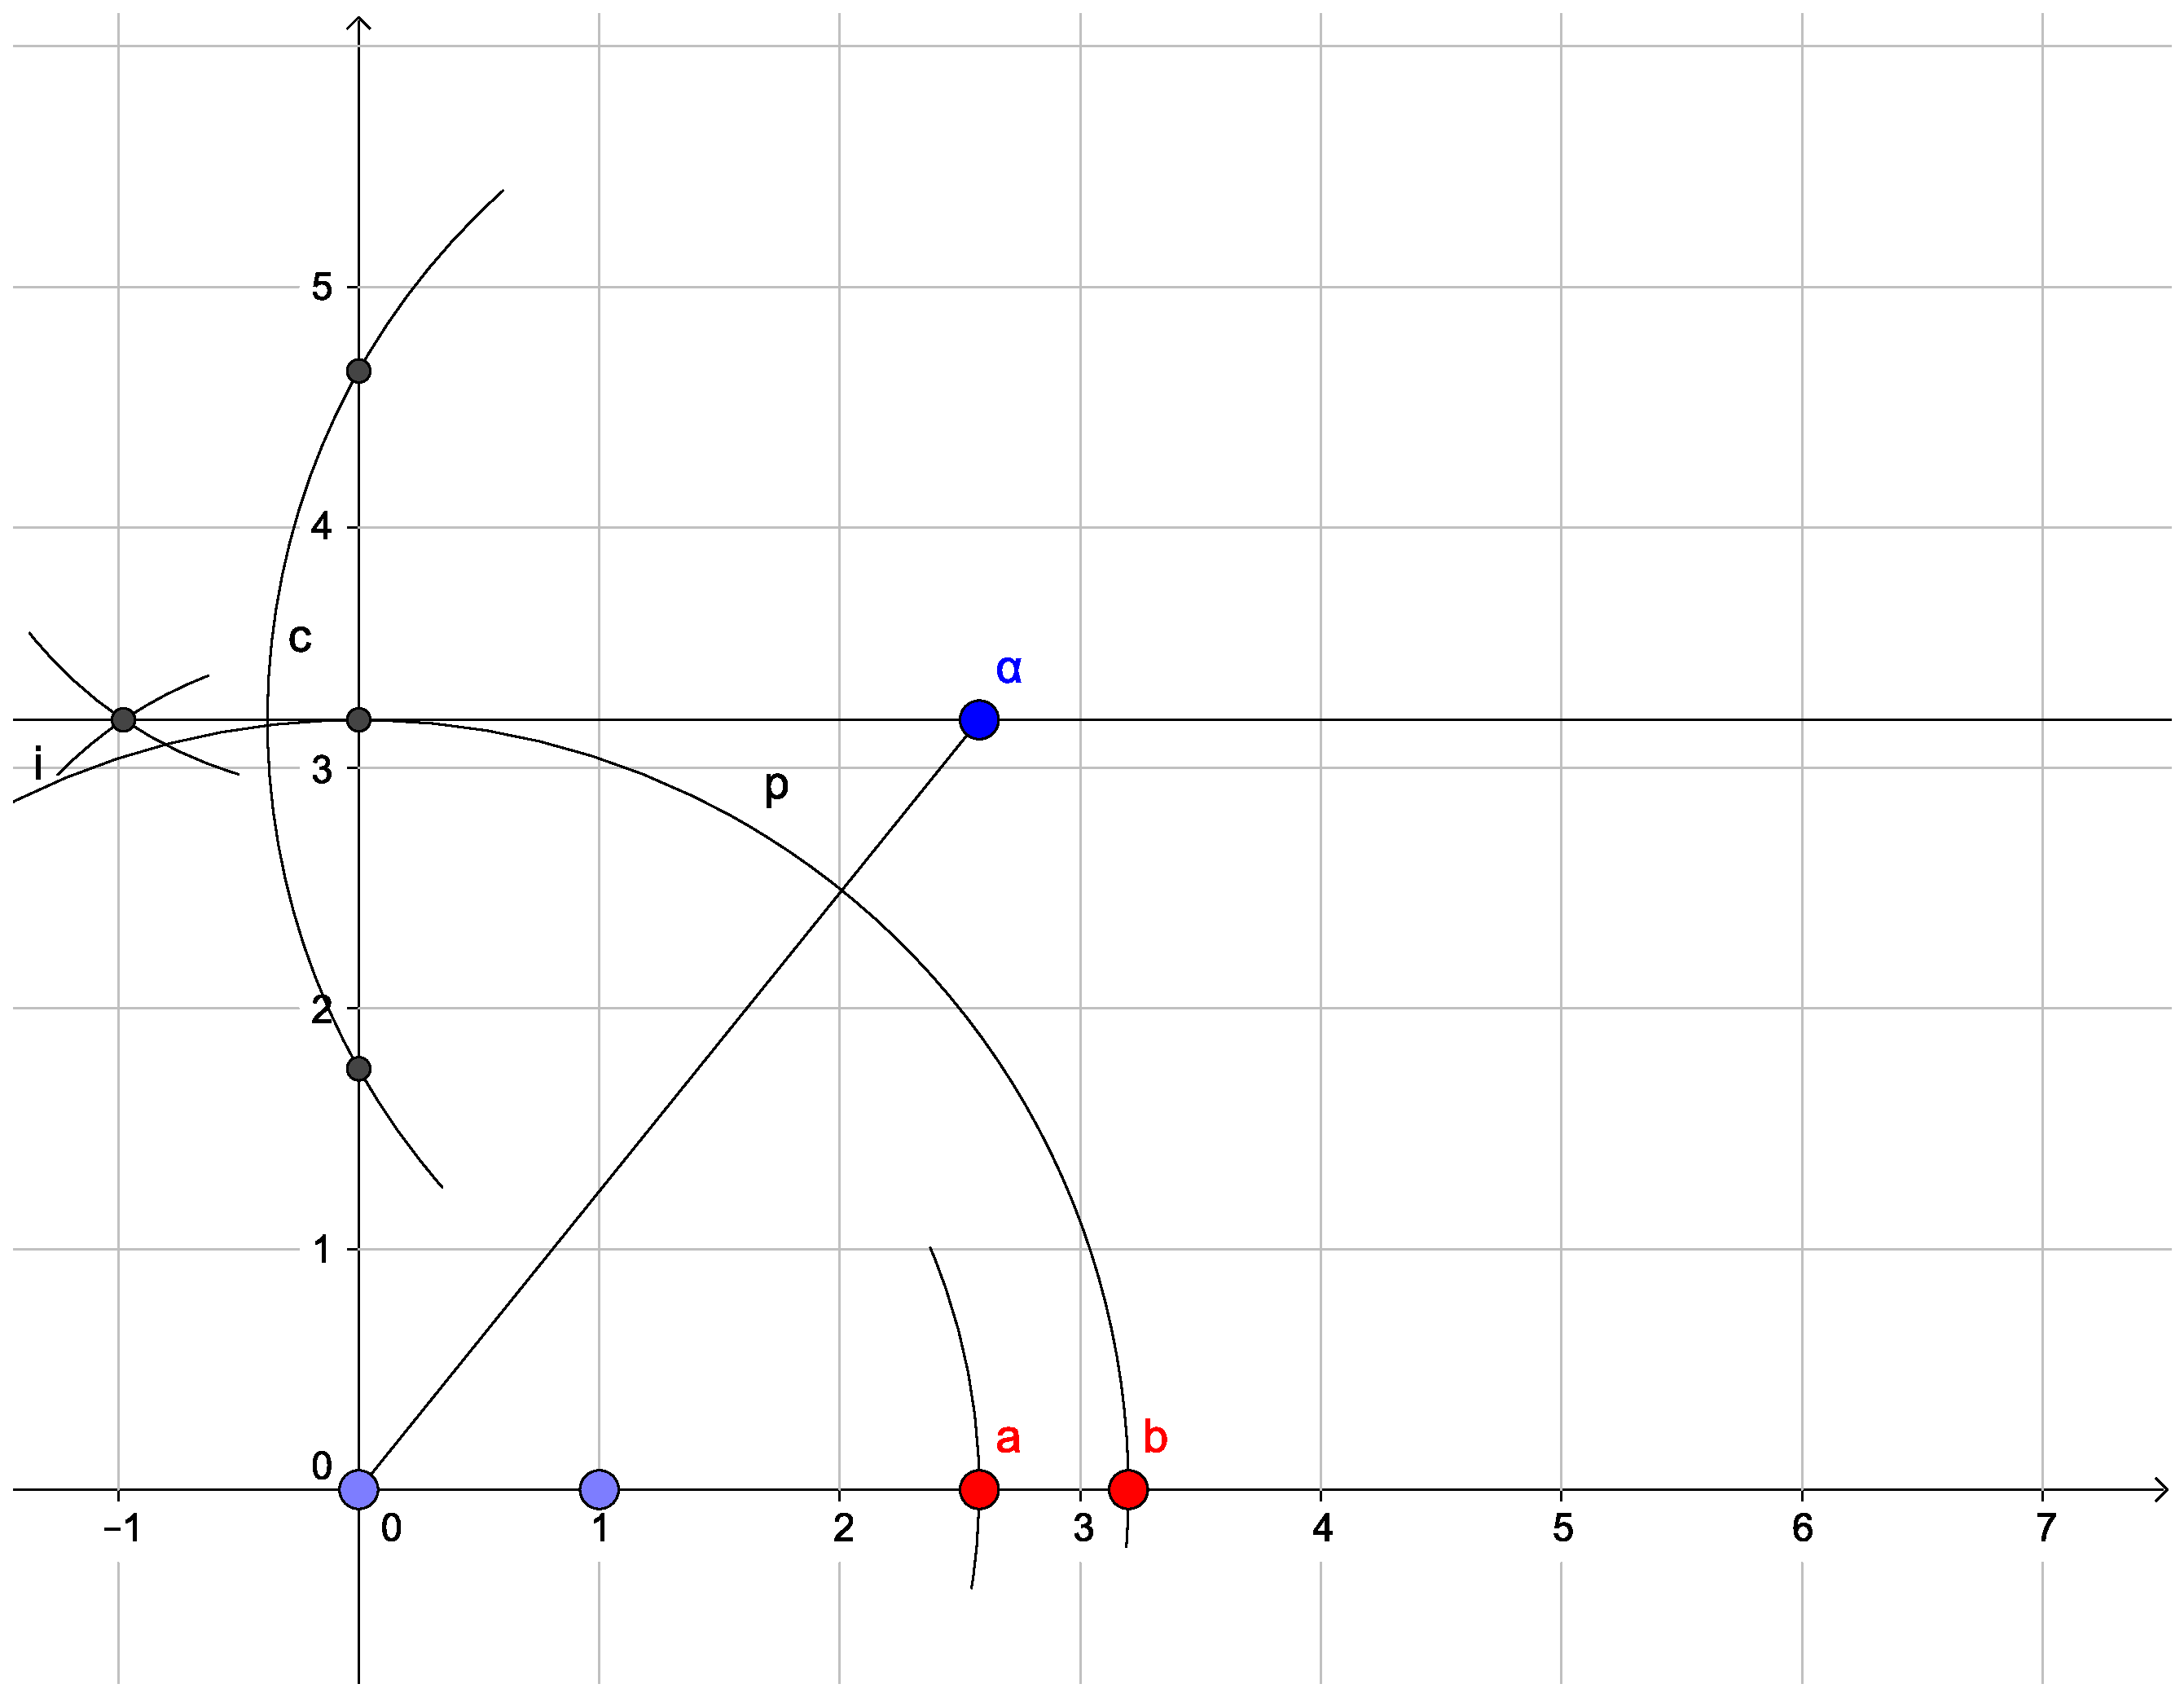
\includegraphics[scale=0.15]{wsp.eps}
\label{fig:dodawanie}
\end{figure}
\end{frame}

\begin{frame}{Liczby Konstruowalne}
\begin{figure}[!htb]
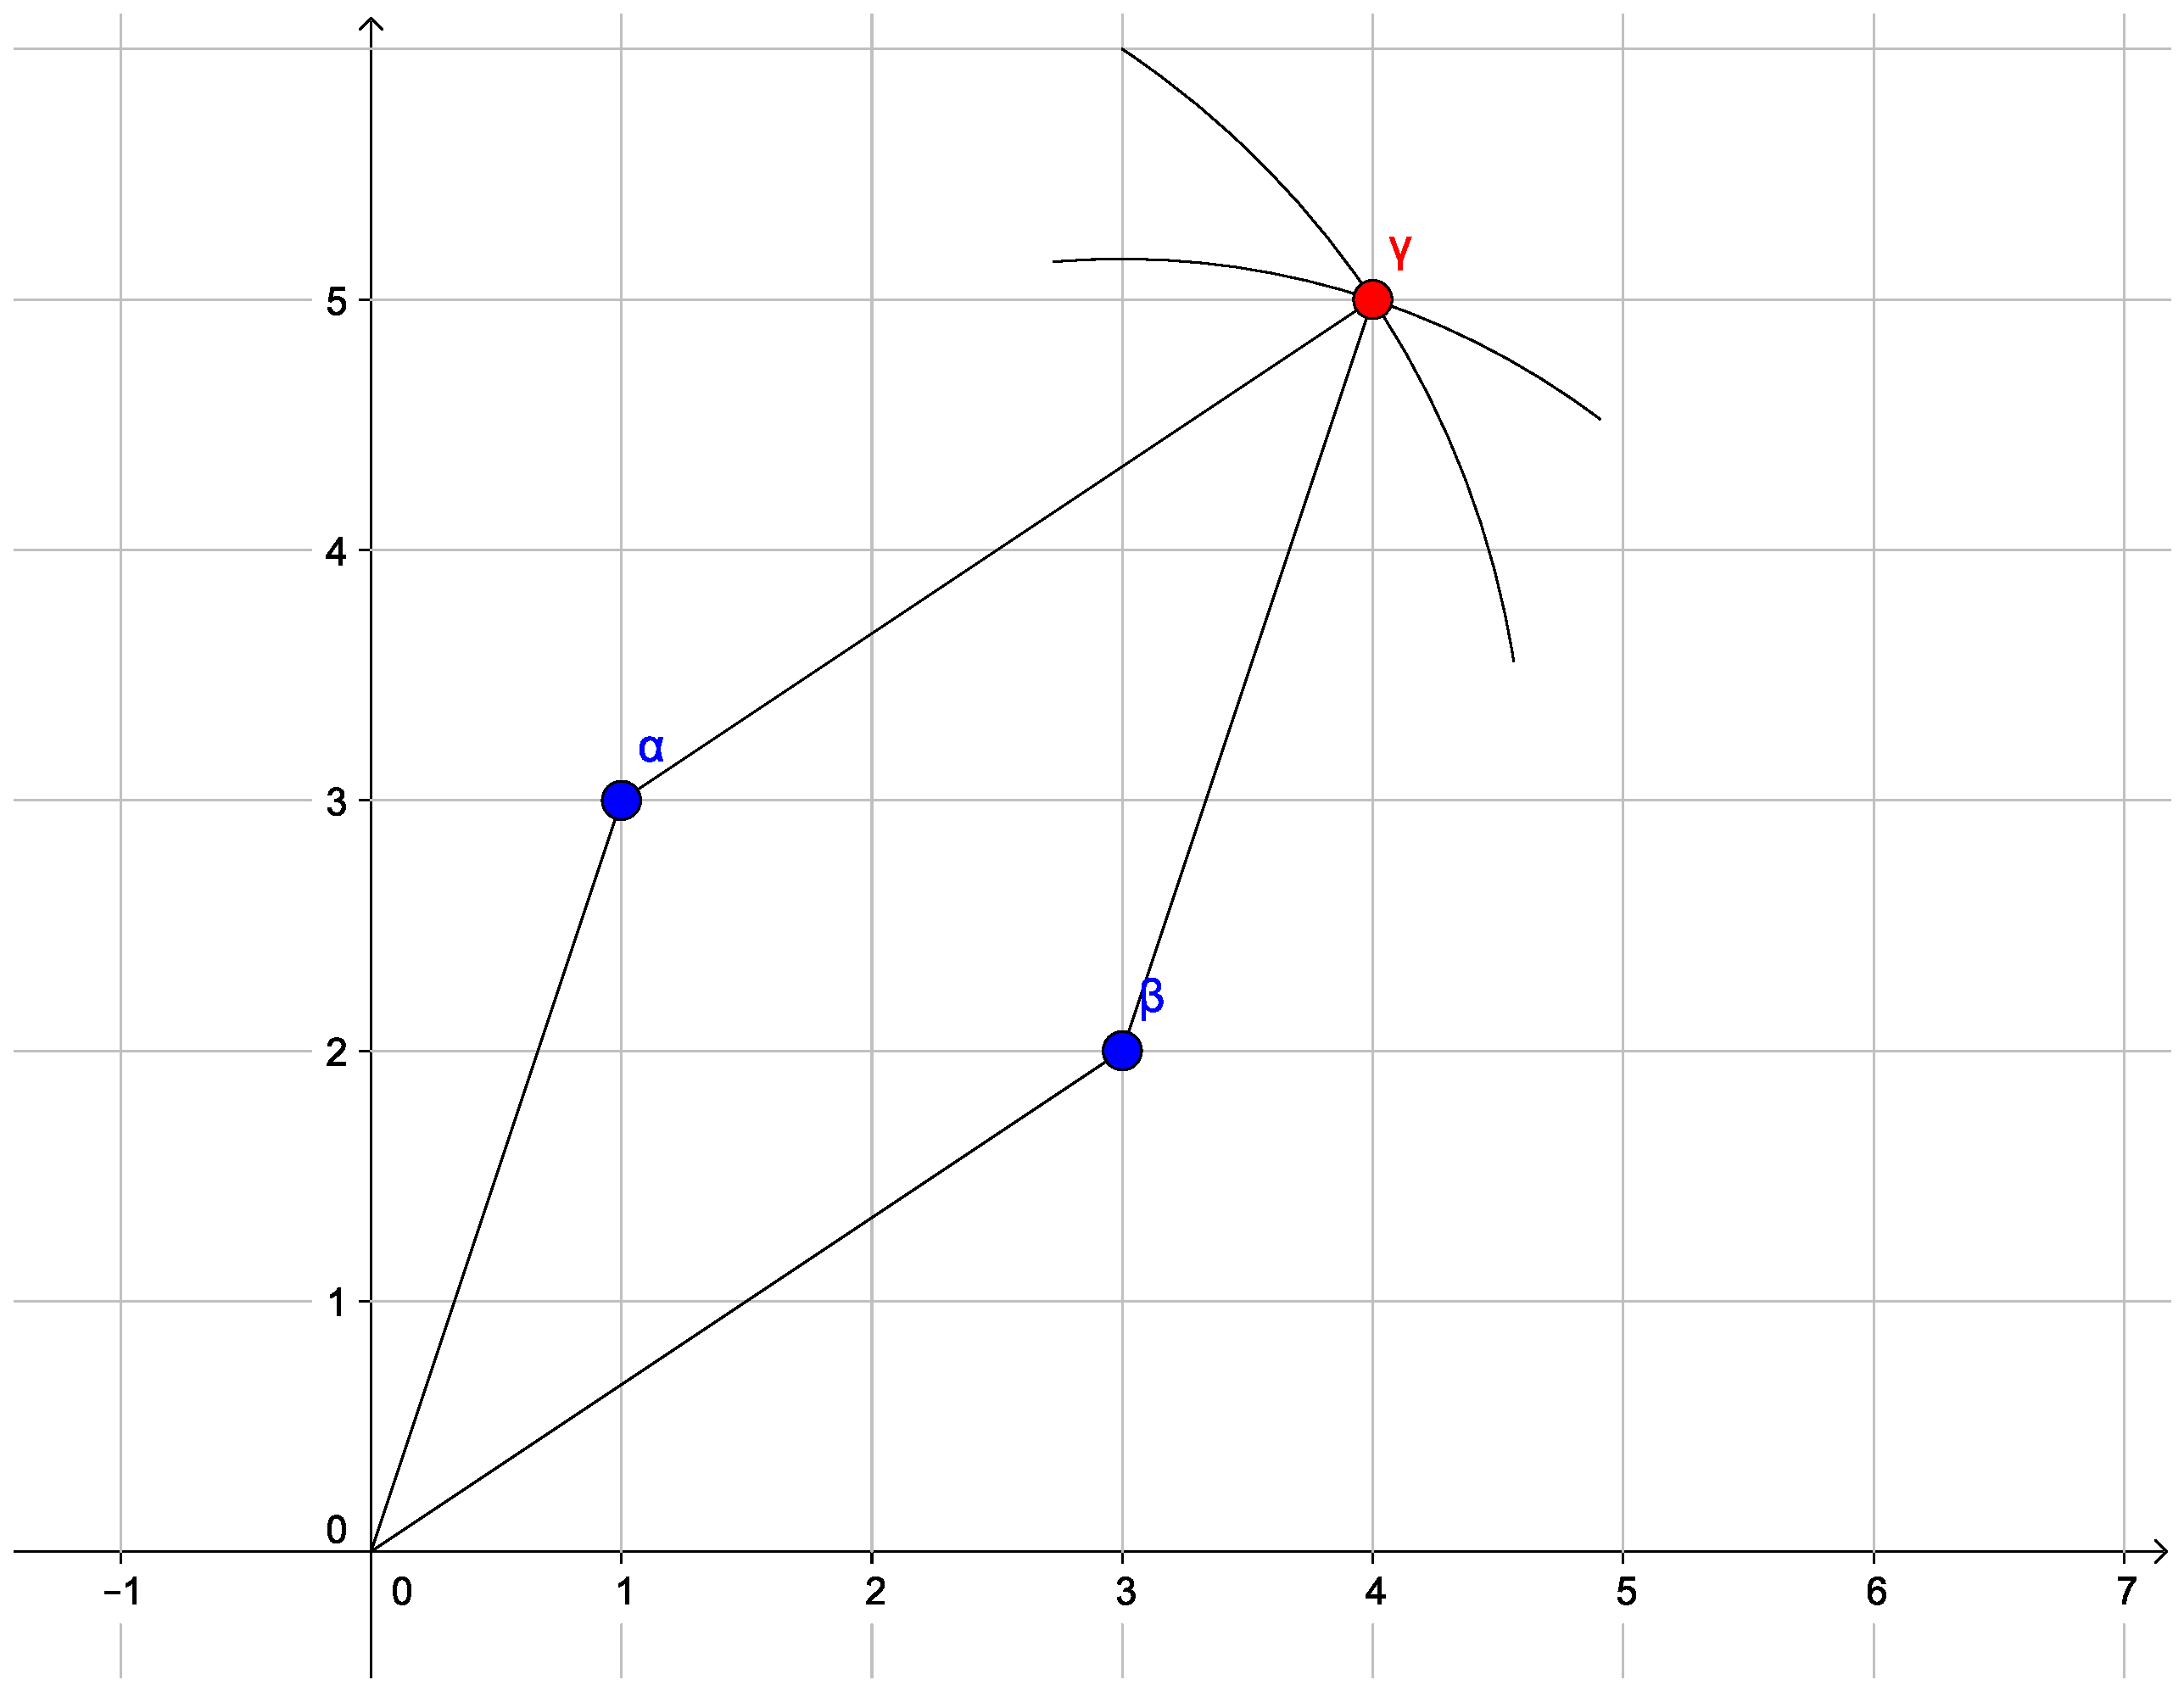
\includegraphics[scale=0.15]{suma.eps}
\label{fig:dodawanie}
\end{figure}
\end{frame}

\begin{frame}{Liczby Konstruowalne}
\begin{Huge}
$$\alpha \cdot \beta=ae^{\theta} \cdot be^{\tau}=(ab)e^{\theta+\tau}$$
\end{Huge}
\end{frame}

\begin{frame}{Liczby Konstruowalne}
\begin{figure}[!htb]
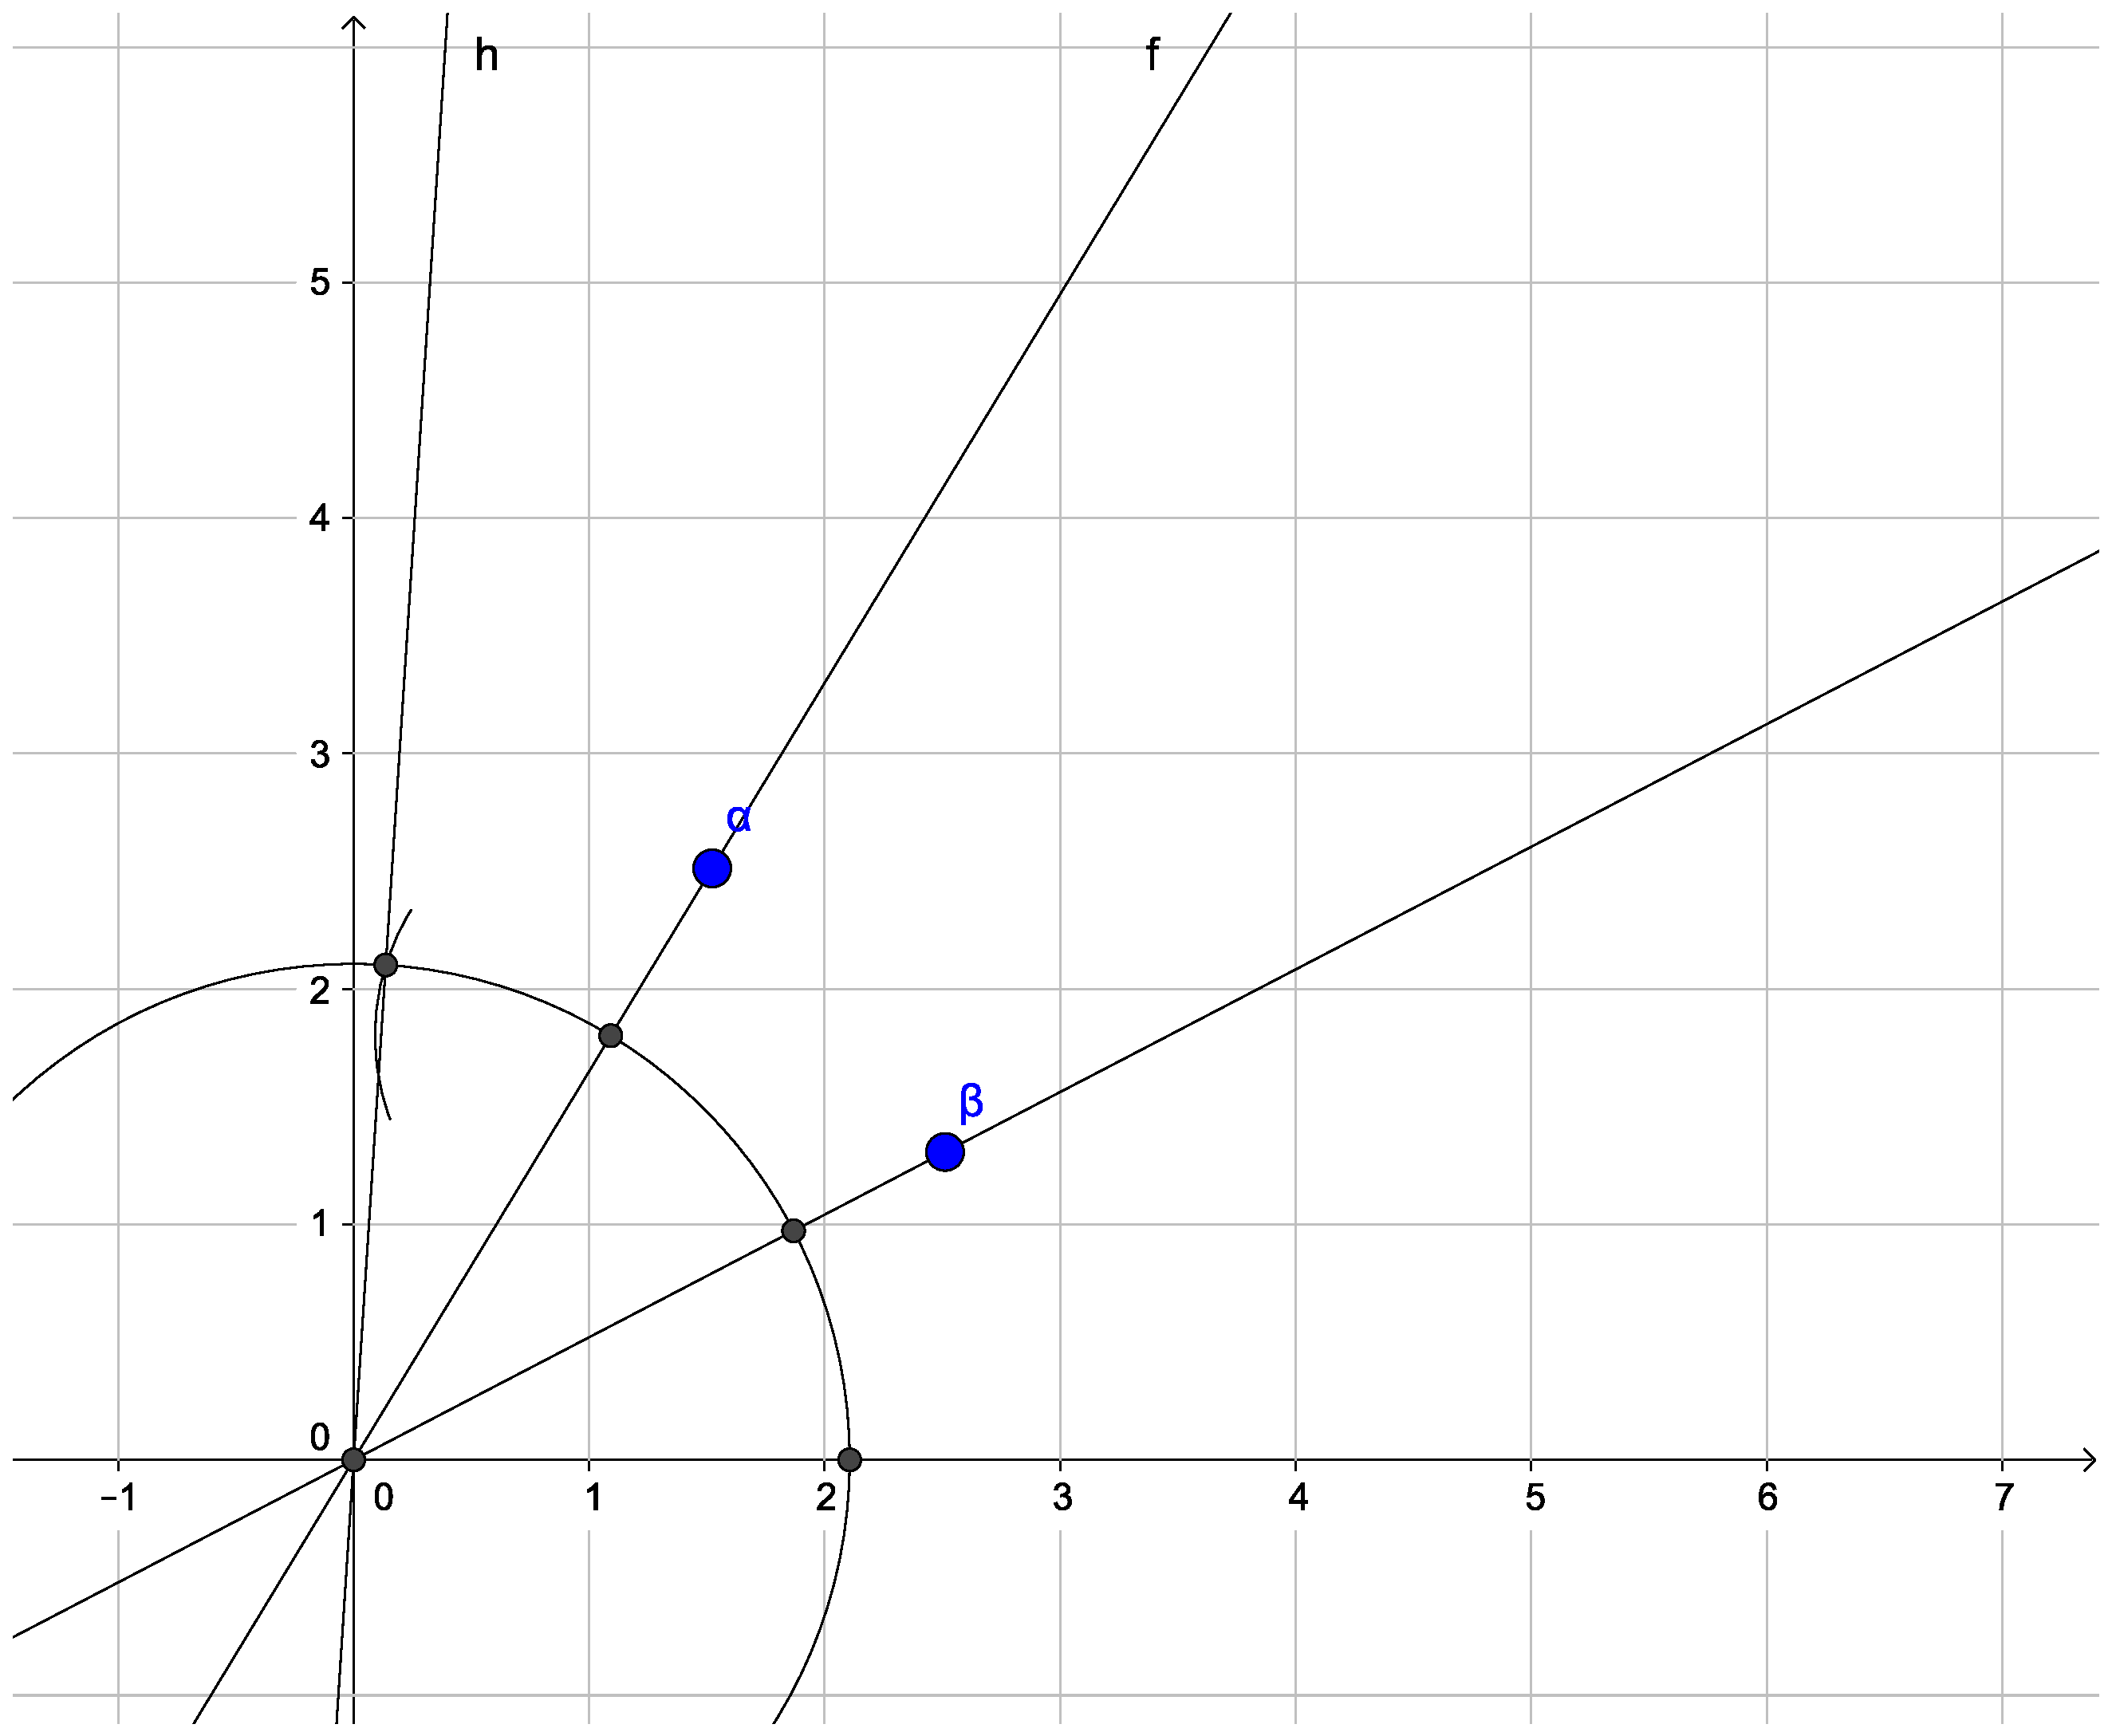
\includegraphics[scale=0.15]{iloczyn1.eps}
\label{fig:iloczyn1}
\end{figure}
\end{frame}

\begin{frame}{Liczby Konstruowalne}
\begin{figure}[!htb]
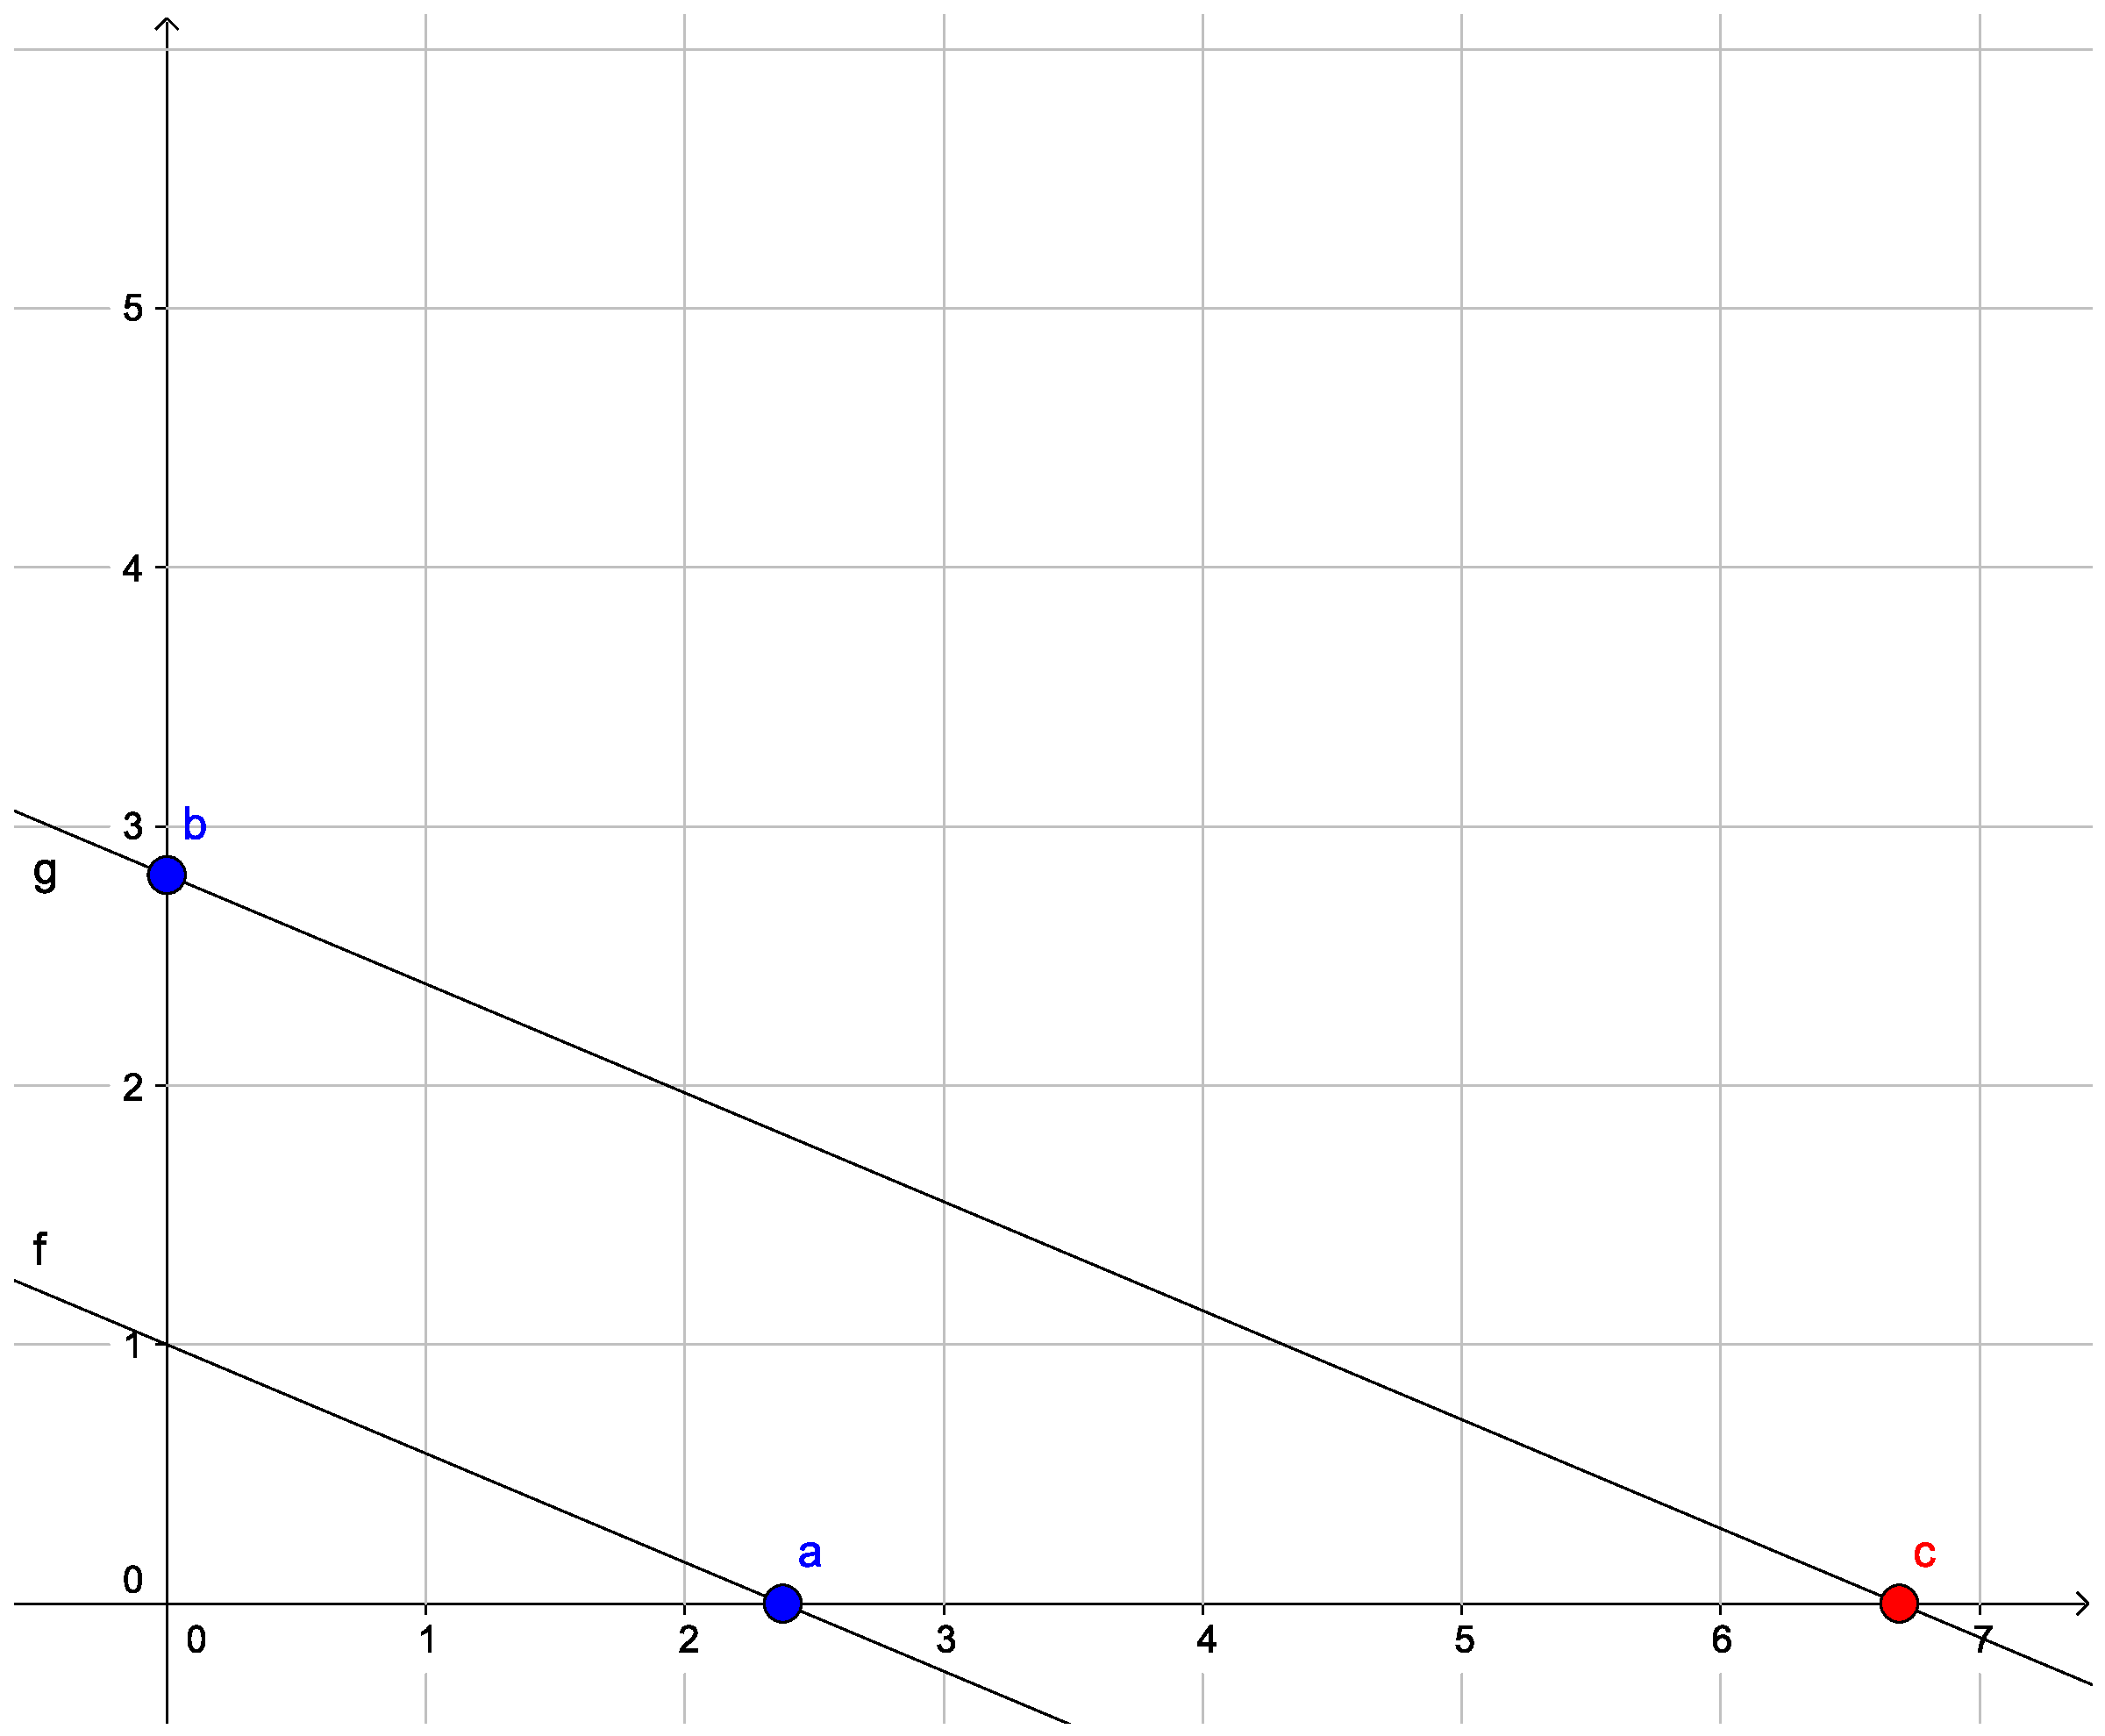
\includegraphics[scale=0.15]{iloczyn2.eps}
\label{fig:iloczyn2}
\end{figure}
\end{frame}

\begin{frame}{Liczby Konstruowalne}
\begin{Huge}
$$\frac{\alpha}{\beta}=\frac{ae^{\theta}}{be^{\tau}}=(\frac{a}{b})e^{\theta-\tau}$$
\end{Huge}
\end{frame}

\begin{frame}{Liczby Konstruowalne}
\begin{figure}[!htb]
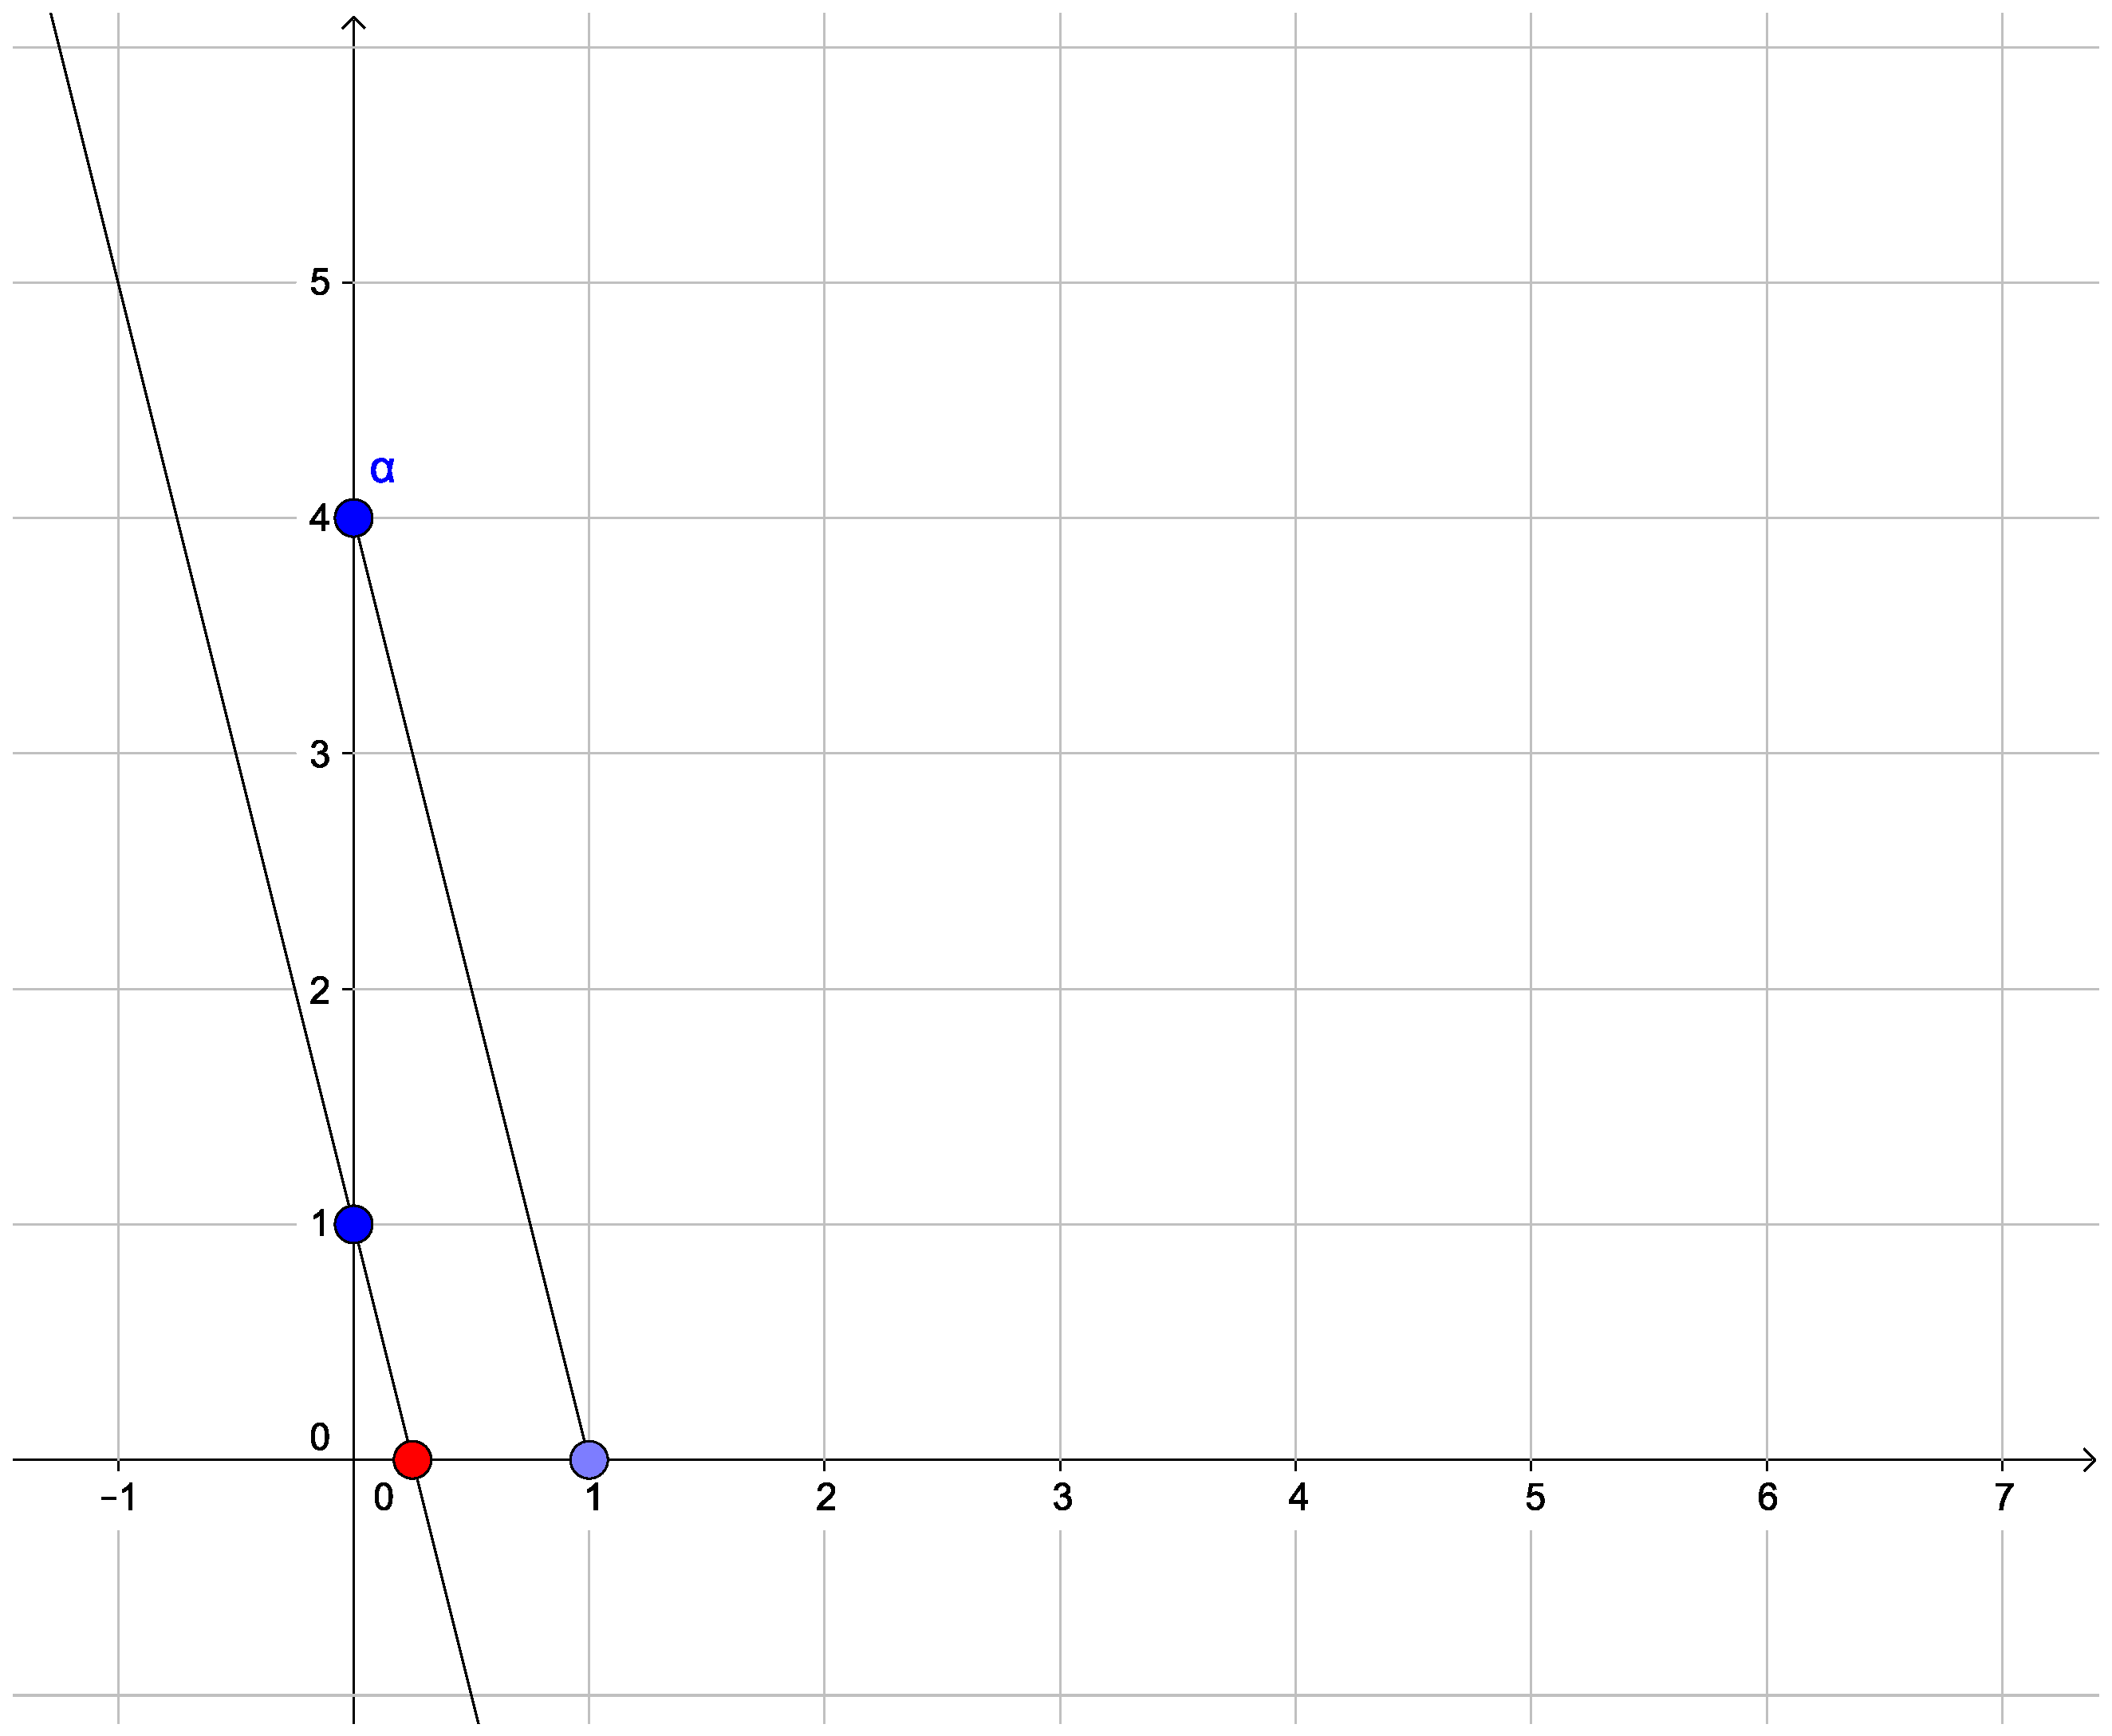
\includegraphics[scale=0.15]{iloraz.eps}
\label{fig:iloraz}
\end{figure}
\end{frame}

\begin{frame}{Liczby Konstruowalne}
\begin{Huge}
$$\sqrt{\alpha}=\sqrt{a}e^{\frac{\theta}{2}}$$
\end{Huge}
\end{frame}

\begin{frame}{Liczby Konstruowalne}
\begin{figure}[!htb]
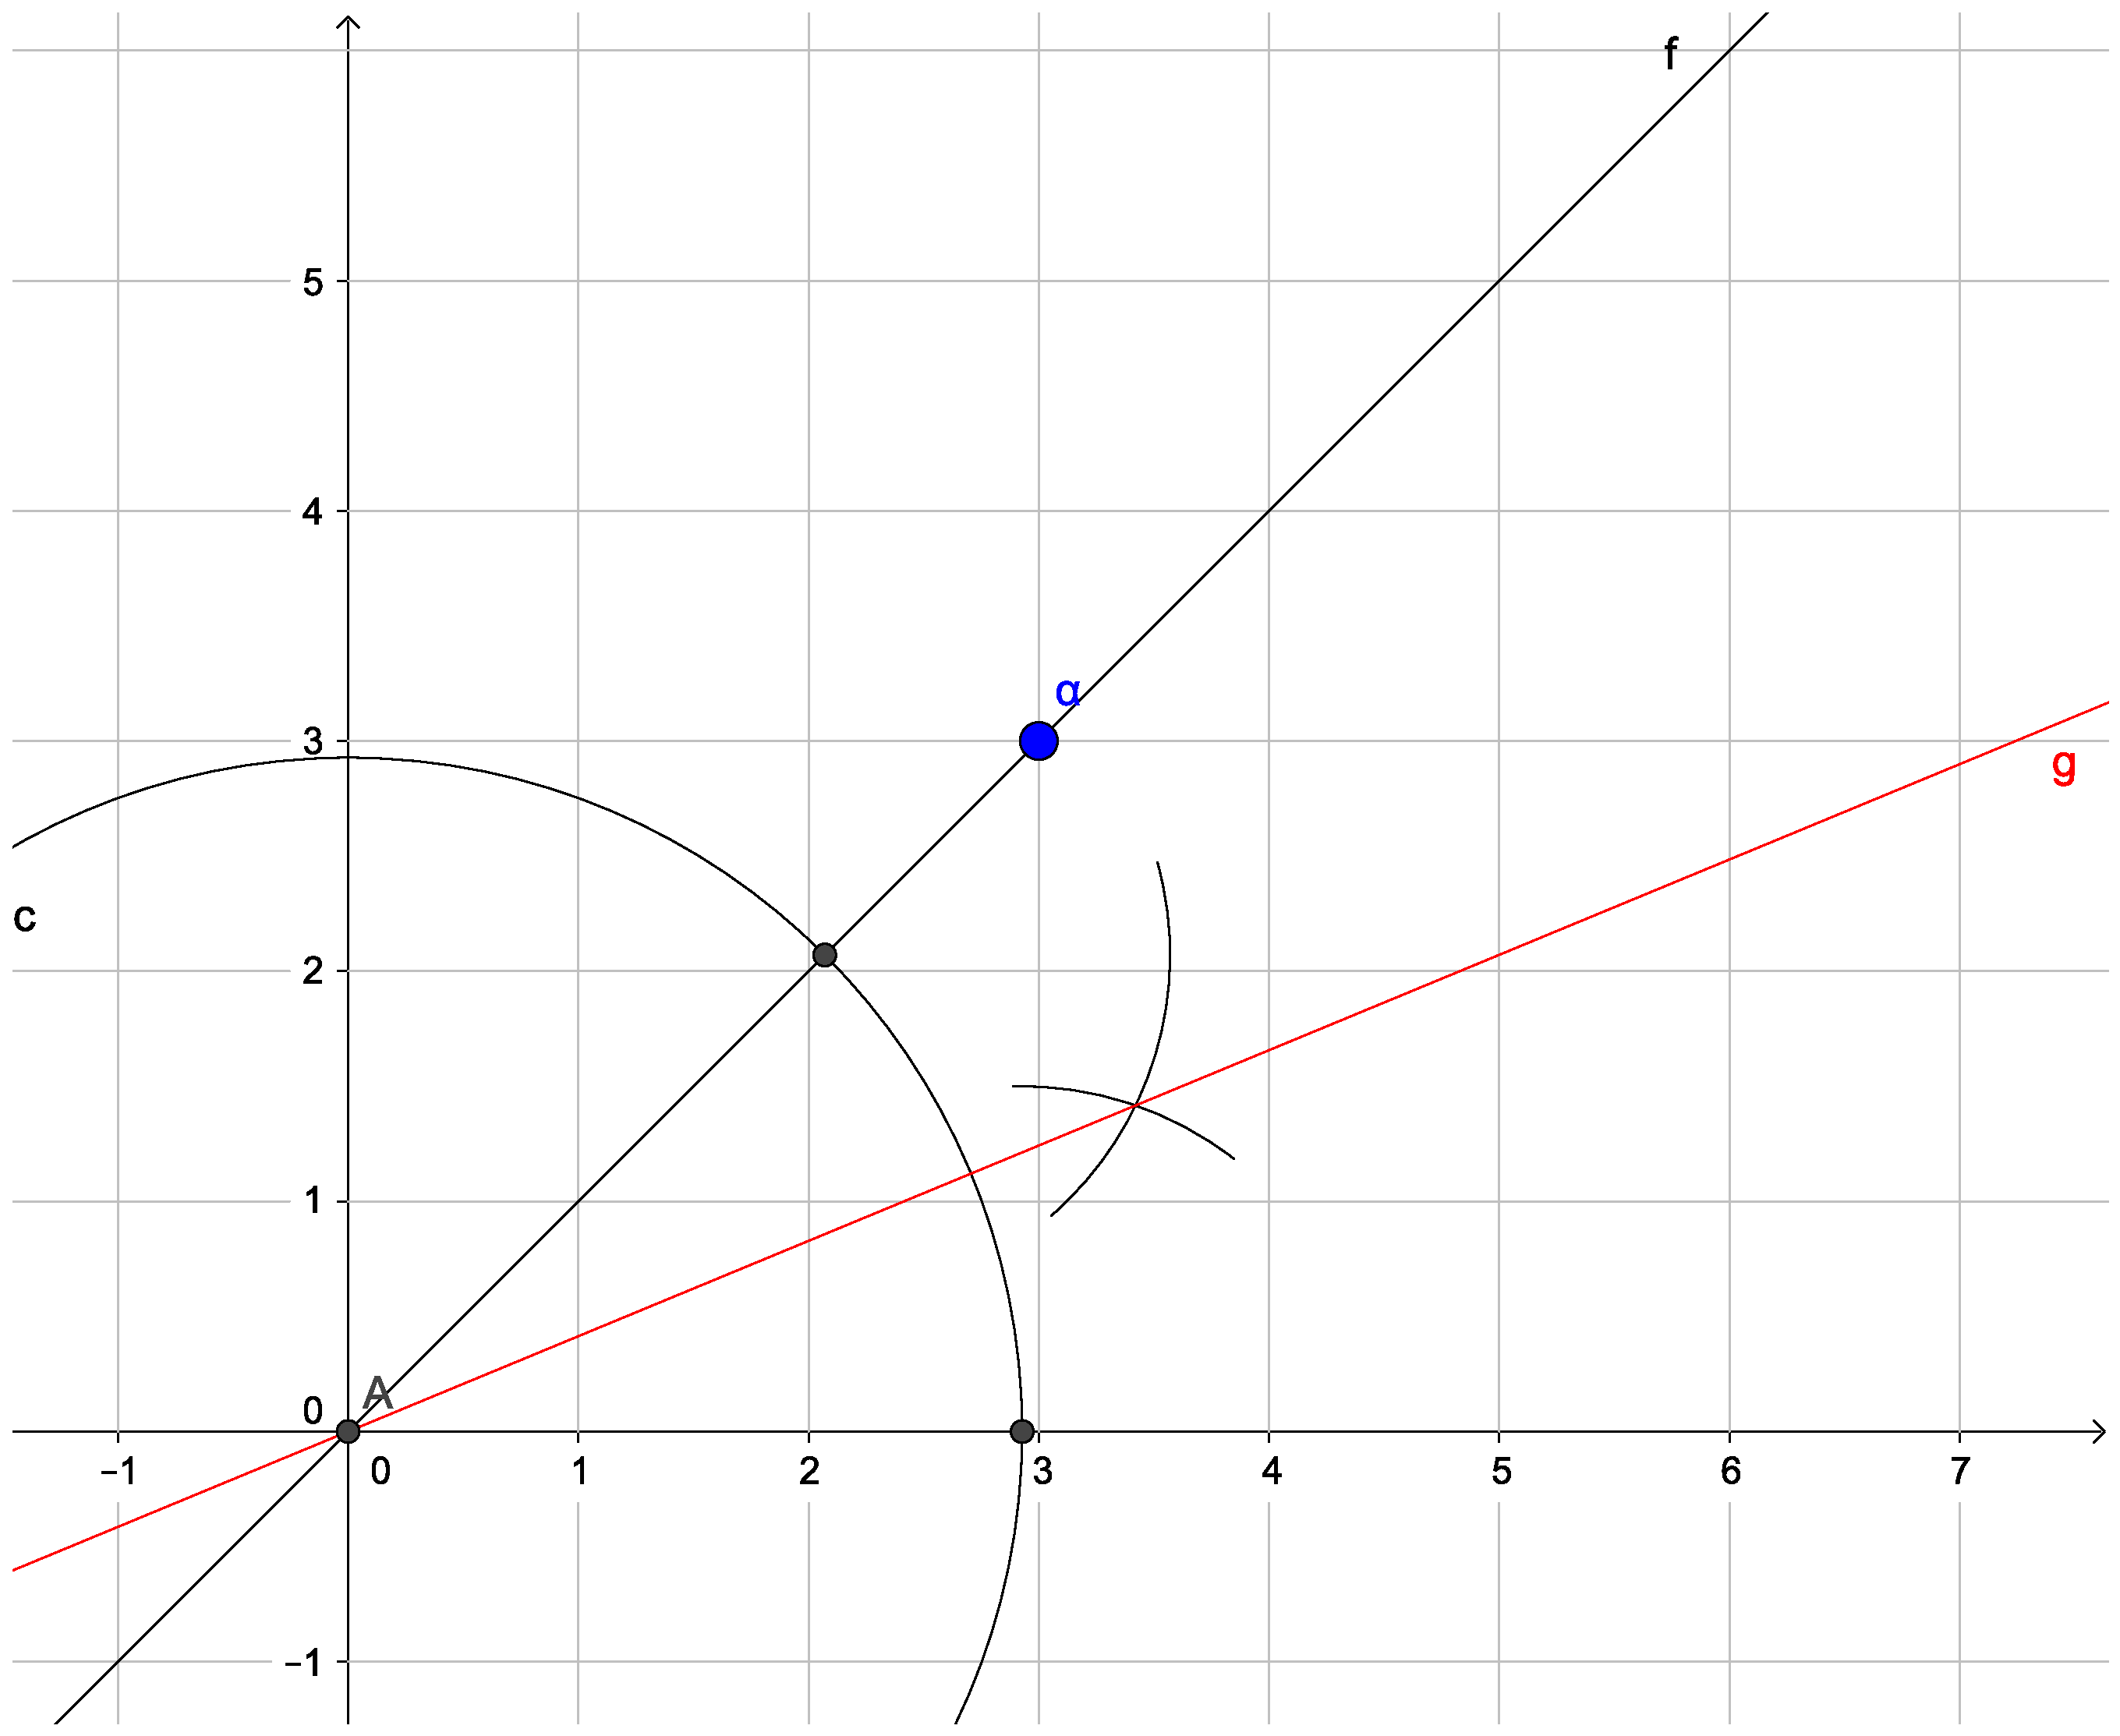
\includegraphics[scale=0.15]{pierwiastek1.eps}
\label{fig:pierwiastek1}
\end{figure}
\end{frame}


\begin{frame}{Liczby Konstruowalne}
\begin{figure}[!htb]
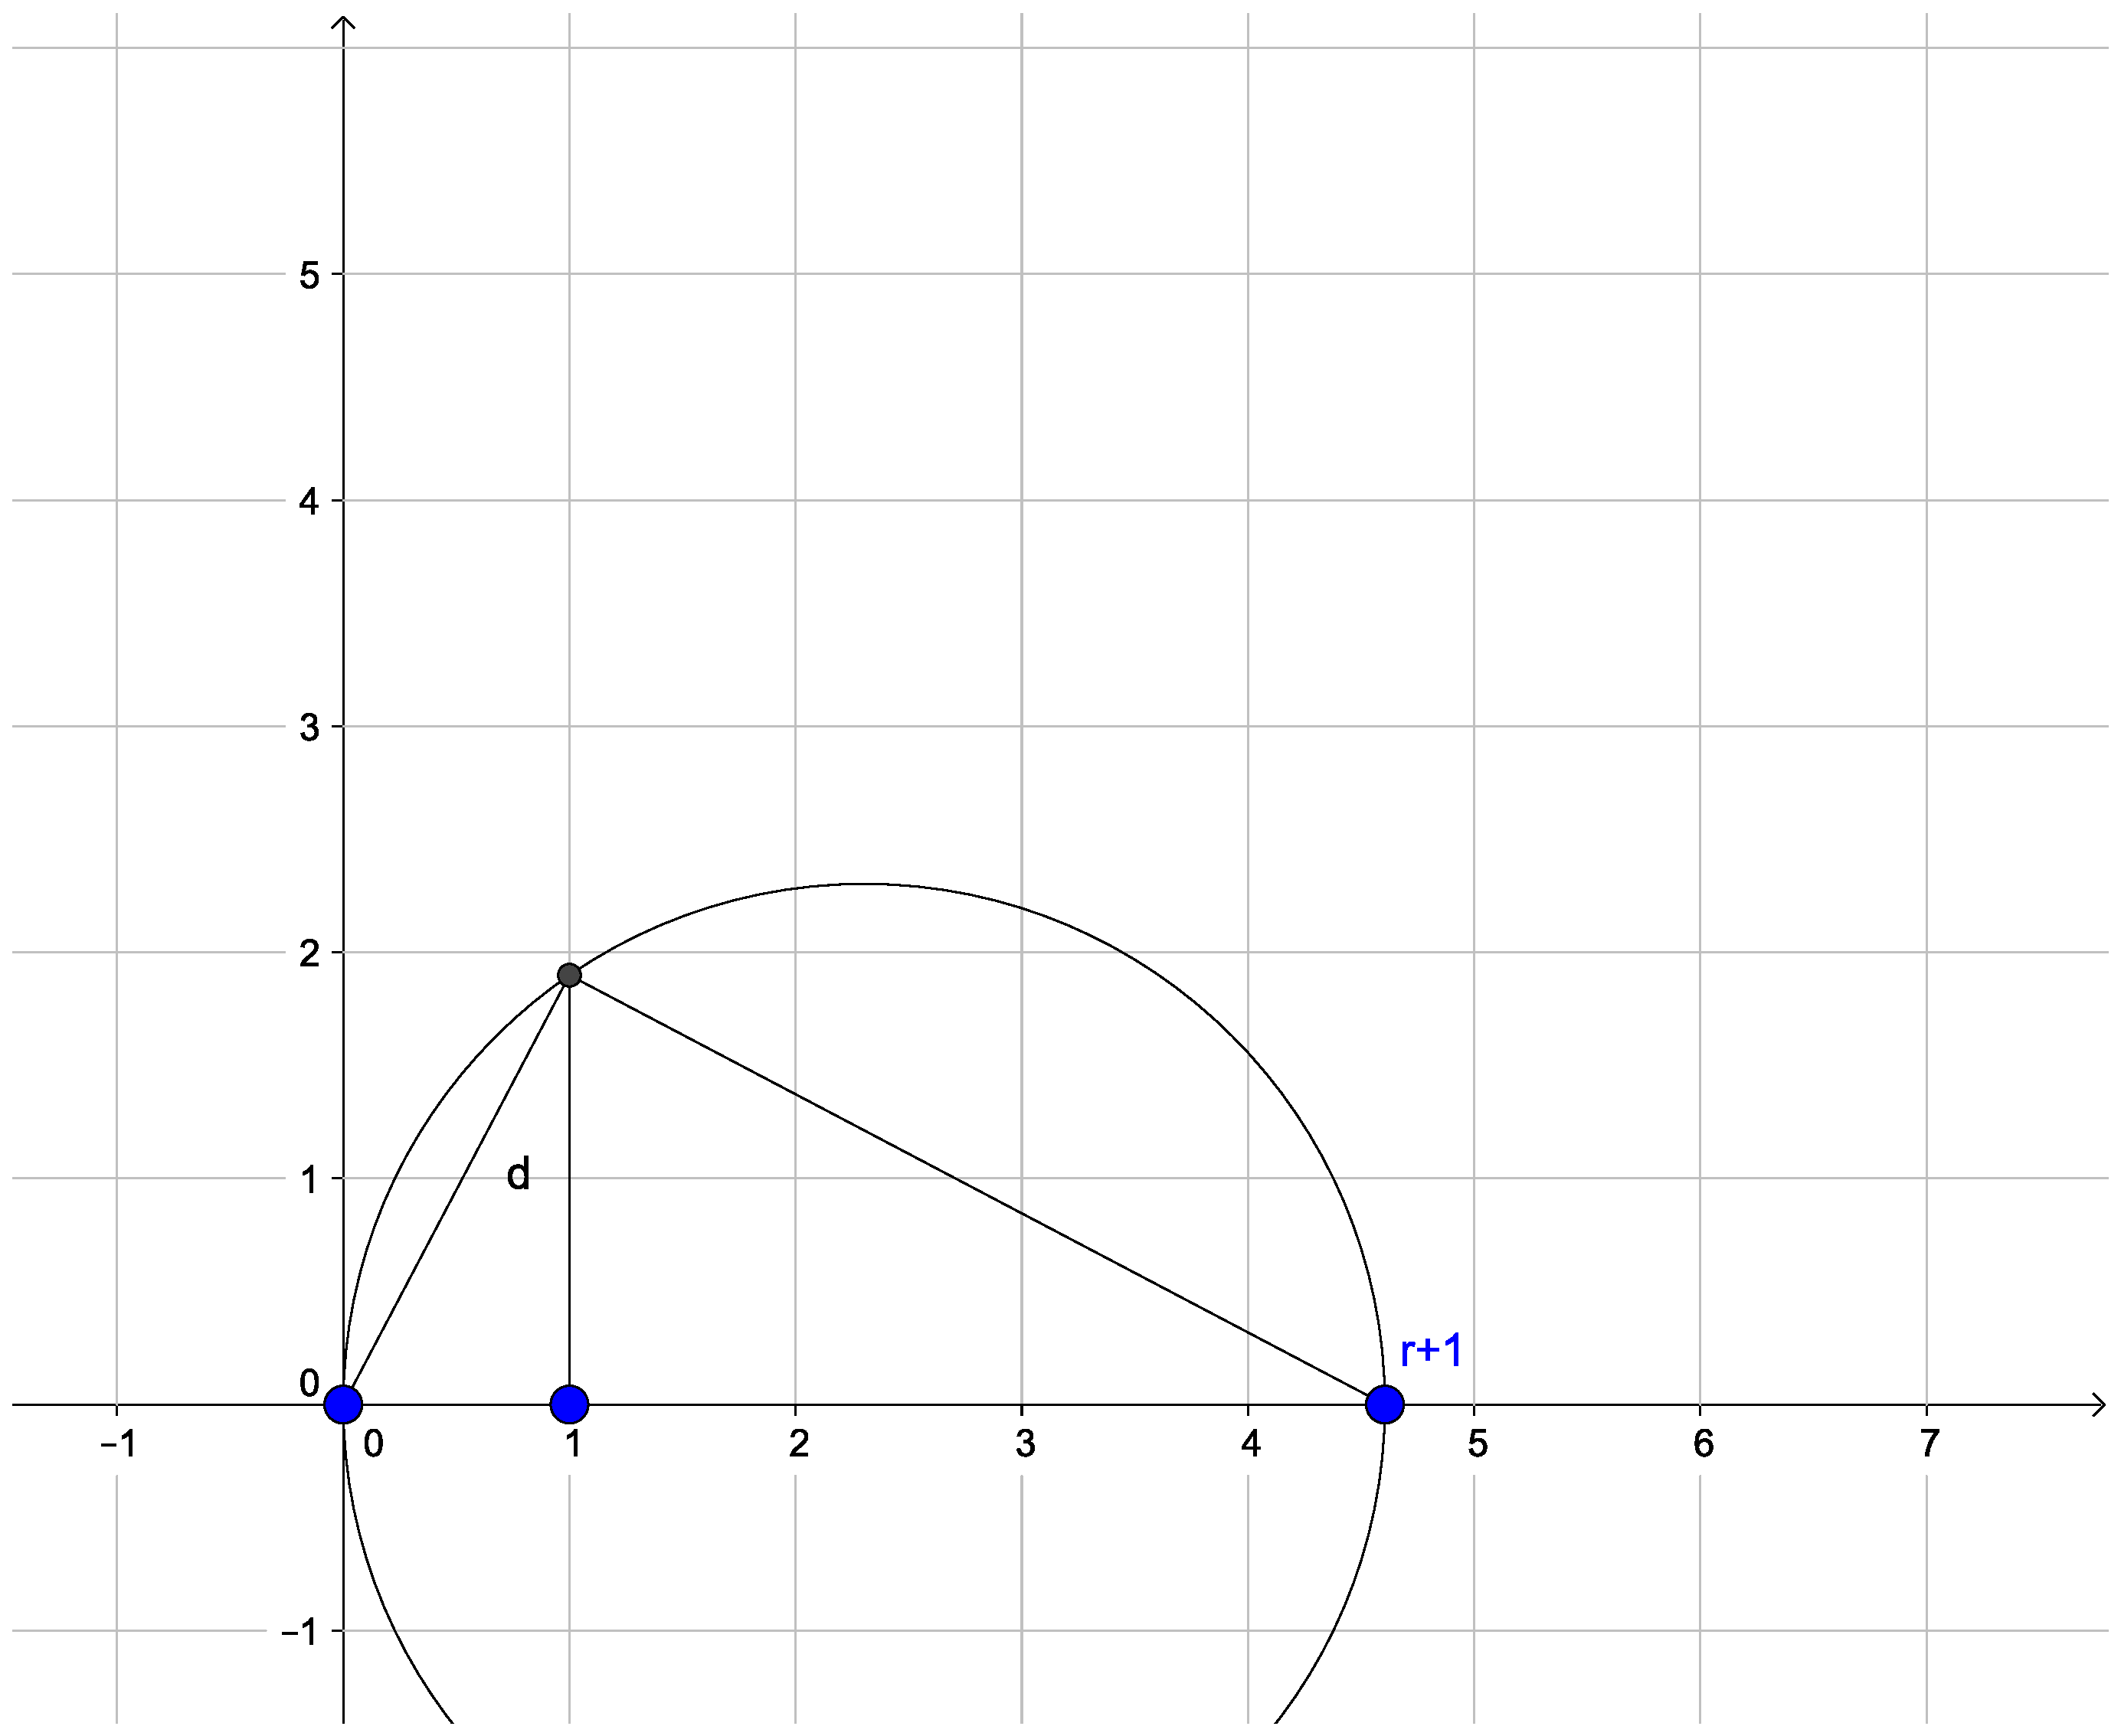
\includegraphics[scale=0.15]{pierwiastek2.eps}
\label{fig:pierwiastek1}
\end{figure}
\end{frame}

\begin{frame}{Liczby Konstruowalne}
\begin{twierdzenie}
Niech $\alpha$ będzie liczbą zespoloną. Wtedy $\alpha\in\mathcal{C}$ wtedy i tylko wtedy, gdy istnieją ciała $$\mathbb{Q}=F_0 \subset F_1 \subset ...\subset F_n \subset \mathbb{C}$$ takie, że $\alpha\in F_n$ i $[F_{i-1}:F_i]=2$ dla $0<i\leqslant n$ 
\end{twierdzenie}
\end{frame}


\begin{frame}{Liczby Konstruowalne}
\begin{proofs}
($\Leftarrow$) Załóżmy, że istnieje $\mathbb{Q}=F_0 \subset ...\subset F_n \subset \mathbb{C}$ gdzie $[F_{i-1}:F_i]=2$. Możemy skorzystać z faktu, że jeżeli $[F_{i-1}:F_i]=2$, to $F_i=F_{i-1}(\sqrt{\alpha_i})$ dla pewnego $\alpha_i\in F_{i-1}$. Poprzez indukcję udowodnimy, że dla $0<i\leqslant n$ $F_i\subset \mathbb{Q}$. Oczywiście $F_0=\mathbb{Q}\subset\mathcal{C}$. Załóżmy, że $F_{i-1}\subset \mathcal{C}$, $F_i=F_{i-1}(\sqrt{\alpha_i})$ . Skoro $\alpha_i\in\mathcal{C}$, to $\sqrt{\alpha_i}\in\mathcal{C}$, stąd $F_i=F_{i-1}(\sqrt{\alpha_i})\in\mathcal{C}$. Zatem $F_n\in\mathcal{C}$.
\end{proofs}
\end{frame}

\begin{frame}{Liczby Konstruowalne}
\begin{proofs}
($\Rightarrow$) $\alpha\in\mathcal{C}$ Udowodnimy, przez stworzenie wieży rozszerzeń
$\mathbb{Q}=F_0 \subset F_1 \subset ...\subset F_n \subset \mathbb{C}$ gdzie $[F_{i-1}:F_i]=2$ takie, że $F_n$ wartości urojone i rzeczywiste liczb, które powstają w trakcie konstrukcji $\alpha$. Przeprowadzimy indukcje po liczbie $N$ użyć aksjomatów P1, P2, P3.
Dla $N=0$ $\alpha=0$ lub $\alpha=1$ zatem $\mathbb{Q}=F_0=F_n$.
\end{proofs}
\end{frame}

\begin{frame}{Liczby Konstruowalne}
\begin{proofs}
Niech $N>1$ i punkt $\alpha$ został otrzymany za pomocą P1, przecięcie się prostych $l_1$, $l_2$. Proste powstały z punktów $\alpha_1$ i $\beta_1$ oraz $\alpha_2$ i $\beta_2$. 
$\alpha_1$, $\beta_1$, $\alpha_2$, $\beta_2$ powstały w co najwyżej $N-1$ krokach, zatem z założenia indukcyjnego istnieje $\mathbb{Q}=F_0 \subset F_1 \subset ...\subset F_n \subset \mathbb{C}$ gdzie $[F_{i-1}:F_i]=2$, że części urojone $\alpha_1$, $\beta_1$, $\alpha_2$, $\beta_2$ należą do $F_n$. Prosta $l_1$ jest opisana równaniem $a_1 x+b_1 y=c_1$, ponieważ $\alpha_1,\beta_1\in F_n$ to $a_1,b_1,c_1\in F_n$. analogicznie równaniem $l_2$ jest $a_2 x+b_2 y=c_2$. $\alpha$ jest punktem przecięcia się $l_1$, $l_2$. Zatem jego części urojone i rzeczywiste rozwiązaniem układu równań:
\begin{equation*}
\begin{matrix}
a_1 x+b_1 y=c_1\\
a_2 x+b_2 y=c_2
\end{matrix}
\end{equation*}
Stąd $\alpha\in F_n$
\end{proofs}
\end{frame}

\begin{frame}{Liczby Konstruowalne}
\begin{proofs}
Niech $N>1$ i punkt $\alpha$ został otrzymany za pomocą P1, przecięcie się prostych $l_1$, $l_2$. Proste powstały z punktów $\alpha_1$ i $\beta_1$ oraz $\alpha_2$ i $\beta_2$. 
$\alpha_1$, $\beta_1$, $\alpha_2$, $\beta_2$ powstały w co najwyżej $N-1$ krokach, zatem z założenia indukcyjnego istnieje $\mathbb{Q}=F_0 \subset F_1 \subset ...\subset F_n \subset \mathbb{C}$ gdzie $[F_{i-1}:F_i]=2$, że części urojone $\alpha_1$, $\beta_1$, $\alpha_2$, $\beta_2$ należą do $F_n$. Prosta $l_1$ jest opisana równaniem $a_1 x+b_1 y=c_1$, ponieważ $\alpha_1,\beta_1\in F_n$ to $a_1,b_1,c_1\in F_n$. analogicznie równaniem $l_2$ jest $a_2 x+b_2 y=c_2$. $\alpha$ jest punktem przecięcia się $l_1$, $l_2$. Zatem jego części urojone i rzeczywiste rozwiązaniem układu równań:
\begin{equation*}
\begin{matrix}
a_1 x+b_1 y=c_1\\
a_2 x+b_2 y=c_2
\end{matrix}
\end{equation*}
Stąd $\alpha\in F_n$
\end{proofs}
\end{frame}

\begin{frame}{Readable Mathematics}

Let $X_1, X_2, \ldots, X_n$ be a sequence of independent and identically distributed random variables with $\text{E}[X_i] = \mu$ and $\text{Var}[X_i] = \sigma^2 < \infty$, and let
$$S_n = \frac{X_1 + X_2 + \cdots + X_n}{n}
      = \frac{1}{n}\sum_{i}^{n} X_i$$
denote their mean. Then as $n$ approaches infinity, the random variables $\sqrt{n}(S_n - \mu)$ converge in distribution to a normal $\mathcal{N}(0, \sigma^2)$.

\end{frame}

\end{document}
